\documentclass[oneside,titlepage,numbers=noenddot,headinclude,%
               footinclude=true,cleardoublepage=empty,abstractoff,BCOR=2mm,%
               paper=a4,fontsize=11pt,ngerman,american]{scrreprt}


% Custom config ===============================================================

% Classic thesis
\usepackage{amssymb}
% ****************************************************************************************************
% classicthesis-config.tex
% formerly known as loadpackages.sty, classicthesis-ldpkg.sty, and classicthesis-preamble.sty
% Use it at the beginning of your ClassicThesis.tex, or as a LaTeX Preamble
% in your ClassicThesis.{tex,lyx} with % ****************************************************************************************************
% classicthesis-config.tex
% formerly known as loadpackages.sty, classicthesis-ldpkg.sty, and classicthesis-preamble.sty
% Use it at the beginning of your ClassicThesis.tex, or as a LaTeX Preamble
% in your ClassicThesis.{tex,lyx} with % ****************************************************************************************************
% classicthesis-config.tex
% formerly known as loadpackages.sty, classicthesis-ldpkg.sty, and classicthesis-preamble.sty
% Use it at the beginning of your ClassicThesis.tex, or as a LaTeX Preamble
% in your ClassicThesis.{tex,lyx} with \input{classicthesis-config}
% ****************************************************************************************************
% If you like the classicthesis, then I would appreciate a postcard.
% My address can be found in the file ClassicThesis.pdf. A collection
% of the postcards I received so far is available online at
% http://postcards.miede.de
% ****************************************************************************************************

% ****************************************************************************************************
% 1. Configure classicthesis for your needs here, e.g., remove "drafting" below
% in order to deactivate the time-stamp on the pages
% ****************************************************************************************************
\PassOptionsToPackage{listings,%drafting,% %eulerchapternumbers,%
				 pdfspacing,eulermath,%floatperchapter,%linedheaders,%
				 subfig,parts,dottedtoc}{classicthesis}
% ********************************************************************
% Available options for classicthesis.sty
% (see ClassicThesis.pdf for more information):
% drafting
% parts nochapters linedheaders
% eulerchapternumbers beramono eulermath pdfspacing minionprospacing
% tocaligned dottedtoc manychapters
% listings floatperchapter subfig
% ********************************************************************

% ********************************************************************
% Triggers for this config
% ********************************************************************
\usepackage{ifthen}
\newboolean{enable-backrefs} % enable backrefs in the bibliography
\setboolean{enable-backrefs}{false} % true false
% ****************************************************************************************************


% ****************************************************************************************************
% 2. Personal data and user ad-hoc commands
% ****************************************************************************************************
\newcommand{\myTitle}{Investigating Why Underrepresented Minorities Choose CS\xspace}
\newcommand{\mySubtitle}{Gaining Insights Into The Effects Of Culturally Responsive Curriculum\xspace}
%\newcommand{\myDegree}{Doktor-Ingenieur (Dr.-Ing.)\xspace}
\newcommand{\myName}{Omoju Miller\xspace}
%\newcommand{\myProf}{Put name here\xspace}
%\newcommand{\myOtherProf}{Put name here\xspace}
%\newcommand{\mySupervisor}{Pierre Geurts\xspace}
%\newcommand{\myFaculty}{Faculty of Applied Sciences\xspace}
%\newcommand{\myDepartment}{Department of EE and CS\xspace}
%\newcommand{\myUni}{University of Liege\xspace}
%\newcommand{\myLocation}{Liege, Belgium\xspace}
%\newcommand{\myTime}{June 2014\xspace}
\newcommand{\myVersion}{version 1.0\xspace}

% ********************************************************************
% Setup, finetuning, and useful commands
% ********************************************************************
\newcounter{dummy} % necessary for correct hyperlinks (to index, bib, etc.)
\newlength{\abcd} % for ab..z string length calculation
\providecommand{\mLyX}{L\kern-.1667em\lower.25em\hbox{Y}\kern-.125emX\@}
\newcommand{\ie}{i.\,e.}
\newcommand{\Ie}{I.\,e.}
\newcommand{\eg}{e.\,g.}
\newcommand{\Eg}{E.\,g.}
% ****************************************************************************************************


% ****************************************************************************************************
% 3. Loading some handy packages
% ****************************************************************************************************
% ********************************************************************
% Packages with options that might require adjustments
% ********************************************************************
%\PassOptionsToPackage{latin9}{inputenc}	% latin9 (ISO-8859-9) = latin1+"Euro sign"
% \usepackage{inputenc}

\usepackage[applemac]{inputenc}

%\PassOptionsToPackage{ngerman,american}{babel}   % change this to your language(s)
% Spanish languages need extra options in order to work with this template
%\PassOptionsToPackage{spanish,es-lcroman}{babel}
 \usepackage{babel}

\PassOptionsToPackage{square,authoryear}{natbib}
 \usepackage{natbib}

\PassOptionsToPackage{fleqn}{amsmath}		% math environments and more by the AMS
 \usepackage{amsmath}

% ********************************************************************
% General useful packages
% ********************************************************************
\PassOptionsToPackage{T1}{fontenc} % T2A for cyrillics
	\usepackage{fontenc}


\usepackage{lipsum}
\usepackage{textcomp} % fix warning with missing font shapes
%\usepackage{scrhack} % fix warnings when using KOMA with listings package
\usepackage{xspace} % to get the spacing after macros right
\usepackage{mparhack} % get marginpar right
%\usepackage{fixltx2e} % fixes some LaTeX stuff
\PassOptionsToPackage{printonlyused,smaller}{acronym}
	\usepackage{acronym} % nice macros for handling all acronyms in the thesis
%\renewcommand*{\acsfont}[1]{\textssc{#1}} % for MinionPro
%\renewcommand{\bflabel}[1]{{#1}\hfill} % fix the list of acronyms
% ****************************************************************************************************


% ****************************************************************************************************
% 4. Setup floats: tables, (sub)figures, and captions
% ****************************************************************************************************
\usepackage{tabularx} % better tables
	\setlength{\extrarowheight}{3pt} % increase table row height
\newcommand{\tableheadline}[1]{\multicolumn{1}{c}{\spacedlowsmallcaps{#1}}}
\newcommand{\myfloatalign}{\centering} % to be used with each float for alignment
\usepackage{caption}
\captionsetup{format=hang,font=small}
\usepackage{subfig}
% ****************************************************************************************************


% ****************************************************************************************************
% 5. Setup code listings
% ****************************************************************************************************
\usepackage{listings}
%\lstset{emph={trueIndex,root},emphstyle=\color{BlueViolet}}%\underbar} % for special keywords
\lstset{language=[LaTeX]Tex,%C++,
    keywordstyle=\color{RoyalBlue},%\bfseries,
    basicstyle=\small\ttfamily,
    %identifierstyle=\color{NavyBlue},
    commentstyle=\color{Green}\ttfamily,
    stringstyle=\rmfamily,
    numbers=none,%left,%
    numberstyle=\scriptsize,%\tiny
    stepnumber=5,
    numbersep=8pt,
    showstringspaces=false,
    breaklines=true,
    frameround=ftff,
    frame=single,
    belowcaptionskip=.75\baselineskip
    %frame=L
}
% ****************************************************************************************************


% ****************************************************************************************************
% 6. PDFLaTeX, hyperreferences and citation backreferences
% ****************************************************************************************************
% ********************************************************************
% Using PDFLaTeX
% ********************************************************************
\PassOptionsToPackage{pdftex,hyperfootnotes=true,pdfpagelabels}{hyperref}
	\usepackage{hyperref}  % backref linktocpage pagebackref
\pdfcompresslevel=9
\pdfadjustspacing=1
\PassOptionsToPackage{pdftex}{graphicx}
	\usepackage{graphicx}

% ********************************************************************
% Setup the style of the backrefs from the bibliography
% (translate the options to any language you use)
% ********************************************************************
\newcommand{\backrefnotcitedstring}{\relax}%(Not cited.)
\newcommand{\backrefcitedsinglestring}[1]{(Cited on page~#1.)}
\newcommand{\backrefcitedmultistring}[1]{(Cited on pages~#1.)}
\ifthenelse{\boolean{enable-backrefs}}%
{%
		\PassOptionsToPackage{hyperpageref}{backref}
		\usepackage{backref} % to be loaded after hyperref package
		   \renewcommand{\backreftwosep}{ and~} % separate 2 pages
		   \renewcommand{\backreflastsep}{, and~} % separate last of longer list
		   \renewcommand*{\backref}[1]{}  % disable standard
		   \renewcommand*{\backrefalt}[4]{% detailed backref
		      \ifcase #1 %
		         \backrefnotcitedstring%
		      \or%
		         \backrefcitedsinglestring{#2}%
		      \else%
		         \backrefcitedmultistring{#2}%
		      \fi}%
}{\relax}

% ********************************************************************
% Hyperreferences
% ********************************************************************
\hypersetup{%
    %draft,	% = no hyperlinking at all (useful in b/w printouts)
    colorlinks=true, linktocpage=true, pdfstartpage=3, pdfstartview=FitV,%
    % uncomment the following line if you want to have black links (e.g., for printing)
    %colorlinks=false, linktocpage=false, pdfborder={0 0 0}, pdfstartpage=3, pdfstartview=FitV,%
    breaklinks=true, pdfpagemode=UseNone, pageanchor=true, pdfpagemode=UseOutlines,%
    plainpages=false, bookmarksnumbered, bookmarksopen=true, bookmarksopenlevel=1,%
    hypertexnames=true, pdfhighlight=/O,%nesting=true,%frenchlinks,%
    urlcolor=webbrown, linkcolor=RoyalBlue, citecolor=webgreen, %pagecolor=RoyalBlue,%
    %urlcolor=Black, linkcolor=Black, citecolor=Black, %pagecolor=Black,%
    pdftitle={\myTitle},%
    pdfauthor={\textcopyright\ \myName},%
    pdfsubject={},%
    pdfkeywords={},%
    pdfcreator={pdfLaTeX},%
    pdfproducer={LaTeX with hyperref and classicthesis}%
}

% ********************************************************************
% Setup autoreferences
% ********************************************************************
% There are some issues regarding autorefnames
% http://www.ureader.de/msg/136221647.aspx
% http://www.tex.ac.uk/cgi-bin/texfaq2html?label=latexwords
% you have to redefine the makros for the
% language you use, e.g., american, ngerman
% (as chosen when loading babel/AtBeginDocument)
% ********************************************************************
\makeatletter
\@ifpackageloaded{babel}%
    {%
       \addto\extrasamerican{%
					\renewcommand*{\figureautorefname}{Figure}%
					\renewcommand*{\tableautorefname}{Table}%
					\renewcommand*{\partautorefname}{Part}%
					\renewcommand*{\chapterautorefname}{Chapter}%
					\renewcommand*{\sectionautorefname}{Section}%
					\renewcommand*{\subsectionautorefname}{Section}%
					\renewcommand*{\subsubsectionautorefname}{Section}%
				}%
       \addto\extrasngerman{%
					\renewcommand*{\paragraphautorefname}{Absatz}%
					\renewcommand*{\subparagraphautorefname}{Unterabsatz}%
					\renewcommand*{\footnoteautorefname}{Fu\"snote}%
					\renewcommand*{\FancyVerbLineautorefname}{Zeile}%
					\renewcommand*{\theoremautorefname}{Theorem}%
					\renewcommand*{\appendixautorefname}{Anhang}%
					\renewcommand*{\equationautorefname}{Gleichung}%
					\renewcommand*{\itemautorefname}{Punkt}%
				}%
			% Fix to getting autorefs for subfigures right (thanks to Belinda Vogt for changing the definition)
			\providecommand{\subfigureautorefname}{\figureautorefname}%
    }{\relax}
\makeatother


% ****************************************************************************************************
% 7. Last calls before the bar closes
% ****************************************************************************************************
% ********************************************************************
% Development Stuff
% ********************************************************************
\listfiles
%\PassOptionsToPackage{l2tabu,orthodox,abort}{nag}
%	\usepackage{nag}
%\PassOptionsToPackage{warning, all}{onlyamsmath}
%	\usepackage{onlyamsmath}

% ********************************************************************
% Last, but not least...
% ********************************************************************
\usepackage{classicthesis}
% ****************************************************************************************************


% ****************************************************************************************************
% 8. Further adjustments (experimental)
% ****************************************************************************************************
% ********************************************************************
% Changing the text area
% ********************************************************************
%\linespread{1.05} % a bit more for Palatino
%\areaset[current]{312pt}{761pt} % 686 (factor 2.2) + 33 head + 42 head \the\footskip
%\setlength{\marginparwidth}{7em}%
%\setlength{\marginparsep}{2em}%

% ********************************************************************
% Using different fonts
% ********************************************************************
%\usepackage[oldstylenums]{kpfonts} % oldstyle notextcomp
%\usepackage[osf]{libertine}
%\usepackage{hfoldsty} % Computer Modern with osf
%\usepackage[light,condensed,math]{iwona}
%\renewcommand{\sfdefault}{iwona}
%\usepackage{lmodern} % <-- no osf support :-(
% \usepackage[T1]{fontenc}
% \usepackage{textcomp}
%\usepackage[urw-garamond]{mathdesign} <-- no osf support :-(
% ****************************************************************************************************

% ****************************************************************************************************
% If you like the classicthesis, then I would appreciate a postcard.
% My address can be found in the file ClassicThesis.pdf. A collection
% of the postcards I received so far is available online at
% http://postcards.miede.de
% ****************************************************************************************************

% ****************************************************************************************************
% 1. Configure classicthesis for your needs here, e.g., remove "drafting" below
% in order to deactivate the time-stamp on the pages
% ****************************************************************************************************
\PassOptionsToPackage{listings,%drafting,% %eulerchapternumbers,%
				 pdfspacing,eulermath,%floatperchapter,%linedheaders,%
				 subfig,parts,dottedtoc}{classicthesis}
% ********************************************************************
% Available options for classicthesis.sty
% (see ClassicThesis.pdf for more information):
% drafting
% parts nochapters linedheaders
% eulerchapternumbers beramono eulermath pdfspacing minionprospacing
% tocaligned dottedtoc manychapters
% listings floatperchapter subfig
% ********************************************************************

% ********************************************************************
% Triggers for this config
% ********************************************************************
\usepackage{ifthen}
\newboolean{enable-backrefs} % enable backrefs in the bibliography
\setboolean{enable-backrefs}{false} % true false
% ****************************************************************************************************


% ****************************************************************************************************
% 2. Personal data and user ad-hoc commands
% ****************************************************************************************************
\newcommand{\myTitle}{Investigating Why Underrepresented Minorities Choose CS\xspace}
\newcommand{\mySubtitle}{Gaining Insights Into The Effects Of Culturally Responsive Curriculum\xspace}
%\newcommand{\myDegree}{Doktor-Ingenieur (Dr.-Ing.)\xspace}
\newcommand{\myName}{Omoju Miller\xspace}
%\newcommand{\myProf}{Put name here\xspace}
%\newcommand{\myOtherProf}{Put name here\xspace}
%\newcommand{\mySupervisor}{Pierre Geurts\xspace}
%\newcommand{\myFaculty}{Faculty of Applied Sciences\xspace}
%\newcommand{\myDepartment}{Department of EE and CS\xspace}
%\newcommand{\myUni}{University of Liege\xspace}
%\newcommand{\myLocation}{Liege, Belgium\xspace}
%\newcommand{\myTime}{June 2014\xspace}
\newcommand{\myVersion}{version 1.0\xspace}

% ********************************************************************
% Setup, finetuning, and useful commands
% ********************************************************************
\newcounter{dummy} % necessary for correct hyperlinks (to index, bib, etc.)
\newlength{\abcd} % for ab..z string length calculation
\providecommand{\mLyX}{L\kern-.1667em\lower.25em\hbox{Y}\kern-.125emX\@}
\newcommand{\ie}{i.\,e.}
\newcommand{\Ie}{I.\,e.}
\newcommand{\eg}{e.\,g.}
\newcommand{\Eg}{E.\,g.}
% ****************************************************************************************************


% ****************************************************************************************************
% 3. Loading some handy packages
% ****************************************************************************************************
% ********************************************************************
% Packages with options that might require adjustments
% ********************************************************************
%\PassOptionsToPackage{latin9}{inputenc}	% latin9 (ISO-8859-9) = latin1+"Euro sign"
% \usepackage{inputenc}

\usepackage[applemac]{inputenc}

%\PassOptionsToPackage{ngerman,american}{babel}   % change this to your language(s)
% Spanish languages need extra options in order to work with this template
%\PassOptionsToPackage{spanish,es-lcroman}{babel}
 \usepackage{babel}

\PassOptionsToPackage{square,authoryear}{natbib}
 \usepackage{natbib}

\PassOptionsToPackage{fleqn}{amsmath}		% math environments and more by the AMS
 \usepackage{amsmath}

% ********************************************************************
% General useful packages
% ********************************************************************
\PassOptionsToPackage{T1}{fontenc} % T2A for cyrillics
	\usepackage{fontenc}


\usepackage{lipsum}
\usepackage{textcomp} % fix warning with missing font shapes
%\usepackage{scrhack} % fix warnings when using KOMA with listings package
\usepackage{xspace} % to get the spacing after macros right
\usepackage{mparhack} % get marginpar right
%\usepackage{fixltx2e} % fixes some LaTeX stuff
\PassOptionsToPackage{printonlyused,smaller}{acronym}
	\usepackage{acronym} % nice macros for handling all acronyms in the thesis
%\renewcommand*{\acsfont}[1]{\textssc{#1}} % for MinionPro
%\renewcommand{\bflabel}[1]{{#1}\hfill} % fix the list of acronyms
% ****************************************************************************************************


% ****************************************************************************************************
% 4. Setup floats: tables, (sub)figures, and captions
% ****************************************************************************************************
\usepackage{tabularx} % better tables
	\setlength{\extrarowheight}{3pt} % increase table row height
\newcommand{\tableheadline}[1]{\multicolumn{1}{c}{\spacedlowsmallcaps{#1}}}
\newcommand{\myfloatalign}{\centering} % to be used with each float for alignment
\usepackage{caption}
\captionsetup{format=hang,font=small}
\usepackage{subfig}
% ****************************************************************************************************


% ****************************************************************************************************
% 5. Setup code listings
% ****************************************************************************************************
\usepackage{listings}
%\lstset{emph={trueIndex,root},emphstyle=\color{BlueViolet}}%\underbar} % for special keywords
\lstset{language=[LaTeX]Tex,%C++,
    keywordstyle=\color{RoyalBlue},%\bfseries,
    basicstyle=\small\ttfamily,
    %identifierstyle=\color{NavyBlue},
    commentstyle=\color{Green}\ttfamily,
    stringstyle=\rmfamily,
    numbers=none,%left,%
    numberstyle=\scriptsize,%\tiny
    stepnumber=5,
    numbersep=8pt,
    showstringspaces=false,
    breaklines=true,
    frameround=ftff,
    frame=single,
    belowcaptionskip=.75\baselineskip
    %frame=L
}
% ****************************************************************************************************


% ****************************************************************************************************
% 6. PDFLaTeX, hyperreferences and citation backreferences
% ****************************************************************************************************
% ********************************************************************
% Using PDFLaTeX
% ********************************************************************
\PassOptionsToPackage{pdftex,hyperfootnotes=true,pdfpagelabels}{hyperref}
	\usepackage{hyperref}  % backref linktocpage pagebackref
\pdfcompresslevel=9
\pdfadjustspacing=1
\PassOptionsToPackage{pdftex}{graphicx}
	\usepackage{graphicx}

% ********************************************************************
% Setup the style of the backrefs from the bibliography
% (translate the options to any language you use)
% ********************************************************************
\newcommand{\backrefnotcitedstring}{\relax}%(Not cited.)
\newcommand{\backrefcitedsinglestring}[1]{(Cited on page~#1.)}
\newcommand{\backrefcitedmultistring}[1]{(Cited on pages~#1.)}
\ifthenelse{\boolean{enable-backrefs}}%
{%
		\PassOptionsToPackage{hyperpageref}{backref}
		\usepackage{backref} % to be loaded after hyperref package
		   \renewcommand{\backreftwosep}{ and~} % separate 2 pages
		   \renewcommand{\backreflastsep}{, and~} % separate last of longer list
		   \renewcommand*{\backref}[1]{}  % disable standard
		   \renewcommand*{\backrefalt}[4]{% detailed backref
		      \ifcase #1 %
		         \backrefnotcitedstring%
		      \or%
		         \backrefcitedsinglestring{#2}%
		      \else%
		         \backrefcitedmultistring{#2}%
		      \fi}%
}{\relax}

% ********************************************************************
% Hyperreferences
% ********************************************************************
\hypersetup{%
    %draft,	% = no hyperlinking at all (useful in b/w printouts)
    colorlinks=true, linktocpage=true, pdfstartpage=3, pdfstartview=FitV,%
    % uncomment the following line if you want to have black links (e.g., for printing)
    %colorlinks=false, linktocpage=false, pdfborder={0 0 0}, pdfstartpage=3, pdfstartview=FitV,%
    breaklinks=true, pdfpagemode=UseNone, pageanchor=true, pdfpagemode=UseOutlines,%
    plainpages=false, bookmarksnumbered, bookmarksopen=true, bookmarksopenlevel=1,%
    hypertexnames=true, pdfhighlight=/O,%nesting=true,%frenchlinks,%
    urlcolor=webbrown, linkcolor=RoyalBlue, citecolor=webgreen, %pagecolor=RoyalBlue,%
    %urlcolor=Black, linkcolor=Black, citecolor=Black, %pagecolor=Black,%
    pdftitle={\myTitle},%
    pdfauthor={\textcopyright\ \myName},%
    pdfsubject={},%
    pdfkeywords={},%
    pdfcreator={pdfLaTeX},%
    pdfproducer={LaTeX with hyperref and classicthesis}%
}

% ********************************************************************
% Setup autoreferences
% ********************************************************************
% There are some issues regarding autorefnames
% http://www.ureader.de/msg/136221647.aspx
% http://www.tex.ac.uk/cgi-bin/texfaq2html?label=latexwords
% you have to redefine the makros for the
% language you use, e.g., american, ngerman
% (as chosen when loading babel/AtBeginDocument)
% ********************************************************************
\makeatletter
\@ifpackageloaded{babel}%
    {%
       \addto\extrasamerican{%
					\renewcommand*{\figureautorefname}{Figure}%
					\renewcommand*{\tableautorefname}{Table}%
					\renewcommand*{\partautorefname}{Part}%
					\renewcommand*{\chapterautorefname}{Chapter}%
					\renewcommand*{\sectionautorefname}{Section}%
					\renewcommand*{\subsectionautorefname}{Section}%
					\renewcommand*{\subsubsectionautorefname}{Section}%
				}%
       \addto\extrasngerman{%
					\renewcommand*{\paragraphautorefname}{Absatz}%
					\renewcommand*{\subparagraphautorefname}{Unterabsatz}%
					\renewcommand*{\footnoteautorefname}{Fu\"snote}%
					\renewcommand*{\FancyVerbLineautorefname}{Zeile}%
					\renewcommand*{\theoremautorefname}{Theorem}%
					\renewcommand*{\appendixautorefname}{Anhang}%
					\renewcommand*{\equationautorefname}{Gleichung}%
					\renewcommand*{\itemautorefname}{Punkt}%
				}%
			% Fix to getting autorefs for subfigures right (thanks to Belinda Vogt for changing the definition)
			\providecommand{\subfigureautorefname}{\figureautorefname}%
    }{\relax}
\makeatother


% ****************************************************************************************************
% 7. Last calls before the bar closes
% ****************************************************************************************************
% ********************************************************************
% Development Stuff
% ********************************************************************
\listfiles
%\PassOptionsToPackage{l2tabu,orthodox,abort}{nag}
%	\usepackage{nag}
%\PassOptionsToPackage{warning, all}{onlyamsmath}
%	\usepackage{onlyamsmath}

% ********************************************************************
% Last, but not least...
% ********************************************************************
\usepackage{classicthesis}
% ****************************************************************************************************


% ****************************************************************************************************
% 8. Further adjustments (experimental)
% ****************************************************************************************************
% ********************************************************************
% Changing the text area
% ********************************************************************
%\linespread{1.05} % a bit more for Palatino
%\areaset[current]{312pt}{761pt} % 686 (factor 2.2) + 33 head + 42 head \the\footskip
%\setlength{\marginparwidth}{7em}%
%\setlength{\marginparsep}{2em}%

% ********************************************************************
% Using different fonts
% ********************************************************************
%\usepackage[oldstylenums]{kpfonts} % oldstyle notextcomp
%\usepackage[osf]{libertine}
%\usepackage{hfoldsty} % Computer Modern with osf
%\usepackage[light,condensed,math]{iwona}
%\renewcommand{\sfdefault}{iwona}
%\usepackage{lmodern} % <-- no osf support :-(
% \usepackage[T1]{fontenc}
% \usepackage{textcomp}
%\usepackage[urw-garamond]{mathdesign} <-- no osf support :-(
% ****************************************************************************************************

% ****************************************************************************************************
% If you like the classicthesis, then I would appreciate a postcard.
% My address can be found in the file ClassicThesis.pdf. A collection
% of the postcards I received so far is available online at
% http://postcards.miede.de
% ****************************************************************************************************

% ****************************************************************************************************
% 1. Configure classicthesis for your needs here, e.g., remove "drafting" below
% in order to deactivate the time-stamp on the pages
% ****************************************************************************************************
\PassOptionsToPackage{listings,%drafting,% %eulerchapternumbers,%
				 pdfspacing,eulermath,%floatperchapter,%linedheaders,%
				 subfig,parts,dottedtoc}{classicthesis}
% ********************************************************************
% Available options for classicthesis.sty
% (see ClassicThesis.pdf for more information):
% drafting
% parts nochapters linedheaders
% eulerchapternumbers beramono eulermath pdfspacing minionprospacing
% tocaligned dottedtoc manychapters
% listings floatperchapter subfig
% ********************************************************************

% ********************************************************************
% Triggers for this config
% ********************************************************************
\usepackage{ifthen}
\newboolean{enable-backrefs} % enable backrefs in the bibliography
\setboolean{enable-backrefs}{false} % true false
% ****************************************************************************************************


% ****************************************************************************************************
% 2. Personal data and user ad-hoc commands
% ****************************************************************************************************
\newcommand{\myTitle}{Investigating Why Underrepresented Minorities Choose CS\xspace}
\newcommand{\mySubtitle}{Gaining Insights Into The Effects Of Culturally Responsive Curriculum\xspace}
%\newcommand{\myDegree}{Doktor-Ingenieur (Dr.-Ing.)\xspace}
\newcommand{\myName}{Omoju Miller\xspace}
%\newcommand{\myProf}{Put name here\xspace}
%\newcommand{\myOtherProf}{Put name here\xspace}
%\newcommand{\mySupervisor}{Pierre Geurts\xspace}
%\newcommand{\myFaculty}{Faculty of Applied Sciences\xspace}
%\newcommand{\myDepartment}{Department of EE and CS\xspace}
%\newcommand{\myUni}{University of Liege\xspace}
%\newcommand{\myLocation}{Liege, Belgium\xspace}
%\newcommand{\myTime}{June 2014\xspace}
\newcommand{\myVersion}{version 1.0\xspace}

% ********************************************************************
% Setup, finetuning, and useful commands
% ********************************************************************
\newcounter{dummy} % necessary for correct hyperlinks (to index, bib, etc.)
\newlength{\abcd} % for ab..z string length calculation
\providecommand{\mLyX}{L\kern-.1667em\lower.25em\hbox{Y}\kern-.125emX\@}
\newcommand{\ie}{i.\,e.}
\newcommand{\Ie}{I.\,e.}
\newcommand{\eg}{e.\,g.}
\newcommand{\Eg}{E.\,g.}
% ****************************************************************************************************


% ****************************************************************************************************
% 3. Loading some handy packages
% ****************************************************************************************************
% ********************************************************************
% Packages with options that might require adjustments
% ********************************************************************
%\PassOptionsToPackage{latin9}{inputenc}	% latin9 (ISO-8859-9) = latin1+"Euro sign"
% \usepackage{inputenc}

\usepackage[applemac]{inputenc}

%\PassOptionsToPackage{ngerman,american}{babel}   % change this to your language(s)
% Spanish languages need extra options in order to work with this template
%\PassOptionsToPackage{spanish,es-lcroman}{babel}
 \usepackage{babel}

\PassOptionsToPackage{square,authoryear}{natbib}
 \usepackage{natbib}

\PassOptionsToPackage{fleqn}{amsmath}		% math environments and more by the AMS
 \usepackage{amsmath}

% ********************************************************************
% General useful packages
% ********************************************************************
\PassOptionsToPackage{T1}{fontenc} % T2A for cyrillics
	\usepackage{fontenc}


\usepackage{lipsum}
\usepackage{textcomp} % fix warning with missing font shapes
%\usepackage{scrhack} % fix warnings when using KOMA with listings package
\usepackage{xspace} % to get the spacing after macros right
\usepackage{mparhack} % get marginpar right
%\usepackage{fixltx2e} % fixes some LaTeX stuff
\PassOptionsToPackage{printonlyused,smaller}{acronym}
	\usepackage{acronym} % nice macros for handling all acronyms in the thesis
%\renewcommand*{\acsfont}[1]{\textssc{#1}} % for MinionPro
%\renewcommand{\bflabel}[1]{{#1}\hfill} % fix the list of acronyms
% ****************************************************************************************************


% ****************************************************************************************************
% 4. Setup floats: tables, (sub)figures, and captions
% ****************************************************************************************************
\usepackage{tabularx} % better tables
	\setlength{\extrarowheight}{3pt} % increase table row height
\newcommand{\tableheadline}[1]{\multicolumn{1}{c}{\spacedlowsmallcaps{#1}}}
\newcommand{\myfloatalign}{\centering} % to be used with each float for alignment
\usepackage{caption}
\captionsetup{format=hang,font=small}
\usepackage{subfig}
% ****************************************************************************************************


% ****************************************************************************************************
% 5. Setup code listings
% ****************************************************************************************************
\usepackage{listings}
%\lstset{emph={trueIndex,root},emphstyle=\color{BlueViolet}}%\underbar} % for special keywords
\lstset{language=[LaTeX]Tex,%C++,
    keywordstyle=\color{RoyalBlue},%\bfseries,
    basicstyle=\small\ttfamily,
    %identifierstyle=\color{NavyBlue},
    commentstyle=\color{Green}\ttfamily,
    stringstyle=\rmfamily,
    numbers=none,%left,%
    numberstyle=\scriptsize,%\tiny
    stepnumber=5,
    numbersep=8pt,
    showstringspaces=false,
    breaklines=true,
    frameround=ftff,
    frame=single,
    belowcaptionskip=.75\baselineskip
    %frame=L
}
% ****************************************************************************************************


% ****************************************************************************************************
% 6. PDFLaTeX, hyperreferences and citation backreferences
% ****************************************************************************************************
% ********************************************************************
% Using PDFLaTeX
% ********************************************************************
\PassOptionsToPackage{pdftex,hyperfootnotes=true,pdfpagelabels}{hyperref}
	\usepackage{hyperref}  % backref linktocpage pagebackref
\pdfcompresslevel=9
\pdfadjustspacing=1
\PassOptionsToPackage{pdftex}{graphicx}
	\usepackage{graphicx}

% ********************************************************************
% Setup the style of the backrefs from the bibliography
% (translate the options to any language you use)
% ********************************************************************
\newcommand{\backrefnotcitedstring}{\relax}%(Not cited.)
\newcommand{\backrefcitedsinglestring}[1]{(Cited on page~#1.)}
\newcommand{\backrefcitedmultistring}[1]{(Cited on pages~#1.)}
\ifthenelse{\boolean{enable-backrefs}}%
{%
		\PassOptionsToPackage{hyperpageref}{backref}
		\usepackage{backref} % to be loaded after hyperref package
		   \renewcommand{\backreftwosep}{ and~} % separate 2 pages
		   \renewcommand{\backreflastsep}{, and~} % separate last of longer list
		   \renewcommand*{\backref}[1]{}  % disable standard
		   \renewcommand*{\backrefalt}[4]{% detailed backref
		      \ifcase #1 %
		         \backrefnotcitedstring%
		      \or%
		         \backrefcitedsinglestring{#2}%
		      \else%
		         \backrefcitedmultistring{#2}%
		      \fi}%
}{\relax}

% ********************************************************************
% Hyperreferences
% ********************************************************************
\hypersetup{%
    %draft,	% = no hyperlinking at all (useful in b/w printouts)
    colorlinks=true, linktocpage=true, pdfstartpage=3, pdfstartview=FitV,%
    % uncomment the following line if you want to have black links (e.g., for printing)
    %colorlinks=false, linktocpage=false, pdfborder={0 0 0}, pdfstartpage=3, pdfstartview=FitV,%
    breaklinks=true, pdfpagemode=UseNone, pageanchor=true, pdfpagemode=UseOutlines,%
    plainpages=false, bookmarksnumbered, bookmarksopen=true, bookmarksopenlevel=1,%
    hypertexnames=true, pdfhighlight=/O,%nesting=true,%frenchlinks,%
    urlcolor=webbrown, linkcolor=RoyalBlue, citecolor=webgreen, %pagecolor=RoyalBlue,%
    %urlcolor=Black, linkcolor=Black, citecolor=Black, %pagecolor=Black,%
    pdftitle={\myTitle},%
    pdfauthor={\textcopyright\ \myName},%
    pdfsubject={},%
    pdfkeywords={},%
    pdfcreator={pdfLaTeX},%
    pdfproducer={LaTeX with hyperref and classicthesis}%
}

% ********************************************************************
% Setup autoreferences
% ********************************************************************
% There are some issues regarding autorefnames
% http://www.ureader.de/msg/136221647.aspx
% http://www.tex.ac.uk/cgi-bin/texfaq2html?label=latexwords
% you have to redefine the makros for the
% language you use, e.g., american, ngerman
% (as chosen when loading babel/AtBeginDocument)
% ********************************************************************
\makeatletter
\@ifpackageloaded{babel}%
    {%
       \addto\extrasamerican{%
					\renewcommand*{\figureautorefname}{Figure}%
					\renewcommand*{\tableautorefname}{Table}%
					\renewcommand*{\partautorefname}{Part}%
					\renewcommand*{\chapterautorefname}{Chapter}%
					\renewcommand*{\sectionautorefname}{Section}%
					\renewcommand*{\subsectionautorefname}{Section}%
					\renewcommand*{\subsubsectionautorefname}{Section}%
				}%
       \addto\extrasngerman{%
					\renewcommand*{\paragraphautorefname}{Absatz}%
					\renewcommand*{\subparagraphautorefname}{Unterabsatz}%
					\renewcommand*{\footnoteautorefname}{Fu\"snote}%
					\renewcommand*{\FancyVerbLineautorefname}{Zeile}%
					\renewcommand*{\theoremautorefname}{Theorem}%
					\renewcommand*{\appendixautorefname}{Anhang}%
					\renewcommand*{\equationautorefname}{Gleichung}%
					\renewcommand*{\itemautorefname}{Punkt}%
				}%
			% Fix to getting autorefs for subfigures right (thanks to Belinda Vogt for changing the definition)
			\providecommand{\subfigureautorefname}{\figureautorefname}%
    }{\relax}
\makeatother


% ****************************************************************************************************
% 7. Last calls before the bar closes
% ****************************************************************************************************
% ********************************************************************
% Development Stuff
% ********************************************************************
\listfiles
%\PassOptionsToPackage{l2tabu,orthodox,abort}{nag}
%	\usepackage{nag}
%\PassOptionsToPackage{warning, all}{onlyamsmath}
%	\usepackage{onlyamsmath}

% ********************************************************************
% Last, but not least...
% ********************************************************************
\usepackage{classicthesis}
% ****************************************************************************************************


% ****************************************************************************************************
% 8. Further adjustments (experimental)
% ****************************************************************************************************
% ********************************************************************
% Changing the text area
% ********************************************************************
%\linespread{1.05} % a bit more for Palatino
%\areaset[current]{312pt}{761pt} % 686 (factor 2.2) + 33 head + 42 head \the\footskip
%\setlength{\marginparwidth}{7em}%
%\setlength{\marginparsep}{2em}%

% ********************************************************************
% Using different fonts
% ********************************************************************
%\usepackage[oldstylenums]{kpfonts} % oldstyle notextcomp
%\usepackage[osf]{libertine}
%\usepackage{hfoldsty} % Computer Modern with osf
%\usepackage[light,condensed,math]{iwona}
%\renewcommand{\sfdefault}{iwona}
%\usepackage{lmodern} % <-- no osf support :-(
% \usepackage[T1]{fontenc}
% \usepackage{textcomp}
%\usepackage[urw-garamond]{mathdesign} <-- no osf support :-(
% ****************************************************************************************************


% Theorems and definitions
\usepackage{amsthm}
\newtheorem{theorem}{Theorem}
\newtheorem{lemma}[theorem]{Lemma}
\newtheorem{proposition}[theorem]{Proposition}
\newtheorem{corollary}[theorem]{Corollary}
\newtheorem{definition}{Definition}

\newtheorem{algorithm}{Algorithm}
\usepackage{algpseudocode}

% Counters
\renewcommand{\labelenumi}{{\color{halfgray}(\alph{enumi})}}
\renewcommand{\labelenumii}{\color{halfgray}{\roman{enumii}.}}
\renewcommand{\labelitemi}{{\color{halfgray}-}}%\raisebox{0.3ex}{\tiny$\blacksquare$}}}

\numberwithin{theorem}{chapter}
\numberwithin{definition}{chapter}
\numberwithin{algorithm}{chapter}
\numberwithin{figure}{chapter}
\numberwithin{table}{chapter}

% Maths
\DeclareMathOperator*{\argmin}{arg\,min}
\DeclareMathOperator*{\argmax}{arg\,max}

\numberwithin{equation}{chapter}
\allowdisplaybreaks

% Shaded boxes
\usepackage{framed}
\newenvironment{remark}[1]{%
  \definecolor{shadecolor}{gray}{0.9}%
  \begin{shaded}{\color{Maroon}\noindent\textsc{#1}}\\%
}{%
  \end{shaded}%
}

% Code snippets
%\usepackage{color}

\usepackage{color}
\definecolor{rulecolor}{rgb}{0.80,0.80,0.80}
\definecolor{bgcolor}{rgb}{1.0,1.0,1.0}
%\newminted{python}{bgcolor=bgcolor}

% Todo
\newcommand{\todo}[1]{\textcolor{red}{[TODO] #1}}

% PS pictures
%\usepackage{pstricks,auto-pst-pdf}

% For the images and graphics
\usepackage{subfig} % For subfigures in floats
\usepackage[section]{placeins}
\makeatletter
 \@ifpackageloaded{tex4ht}{%
\usepackage[dvips]{color,graphicx}
    \usepackage[tex4ht]{hyperref}
    }{%
      \usepackage[pdftex]{graphicx}
      \usepackage{hyperref}
          }
\makeatother
\graphicspath{ {figures/} } %Path to images


% Landscape tables
\usepackage{rotating}

% Checkmarks
\usepackage{pifont}% http://ctan.org/pkg/pifont
\newcommand{\cmark}{\ding{51}}%
\newcommand{\xmark}{\ding{55}}%

% Wide tables
\usepackage{ltablex}


% -----------------------------------------------------------------------------

\begin{document}
\frenchspacing
\raggedbottom
\selectlanguage{american}
\pagenumbering{roman}
\pagestyle{plain}


% Front pages =================================================================
% Front page ==================================================================

\begin{titlepage}
    \begin{addmargin}[-1cm]{-3cm}
    \begin{center}
        \large
        {\Large \textsc{AltAI}}\\[1ex]
    
      

        \vfill

        Rough Draft ASEE 2016\\ \vskip1cm
        \rule{14cm}{0.4pt}\\ \bigskip
        \begingroup
            \Large
            \color{Maroon}\spacedallcaps{\myTitle} \\ \bigskip
        \endgroup
        \spacedlowsmallcaps{\mySubtitle} \\ \bigskip
        \rule{14cm}{0.4pt}\\ \vskip1cm
        by \textsc{Omoju Miller}

        \vfill
        \vfill
        \vfill

       
        \hfill \today
    \end{center}
    \vspace{-3.5cm}
  \end{addmargin}
\end{titlepage}


% Content =====================================================================
\pagenumbering{arabic}

\cleardoublepage

%----------------------------------------------------------------------------------------
%  CHAPTER CONTENTS
%----------------------------------------------------------------------------------------
\chapter*{Why do URMs Choose CS}

%----------------------------------------------------------------------------------------
%  PAPER CONTENTS
%----------------------------------------------------------------------------------------
\section*{Introduction}

One of most pressing question for my generation to answer is that of equalizing participation in our economic life, and particularly in the new technical economy. In the field of computer science (CS), there is a near absence of women and underrepresented ethnic minorities (African Americans, Hispanics, Native Americans, Pacific Islanders and persons with disabilities) \citep{Trauth:2012:UUT:2132176.2132184,Gurer2002,Zweben2010,Foundation:2013qy}. This statement should be alarming to anyone, because it means that nearly 70\%---women, ethnic minorities and persons with disabilities---of the American workforce is not fully engaged in the technology sector. 

As can be seen from figure \ref{femSTEMgrad}, in the nineteen eighties, more than 30\% of all graduating universities CS majors were women. By 2010, that number was less than 20\%. Two folk theories have been historically offered to explain this phenomenon. The first states that women are not good at maths, while the second states that maths is a strong indicator of CS aptitude. These two folk theories are tied together to explain the low participation rates of women in CS. Nevertheless, from figure \ref{satMathMajor}, we see that intended CS majors do not have the strongest maths SAT scores \cite{Kinnunen:2006:WSD:1151588.1151604}. From data, we see that this lack of \textit{alleged} maths aptitude alone can not explain the low participation rates of women in CS.
\begin{figure}[hbtp]
  \centering
  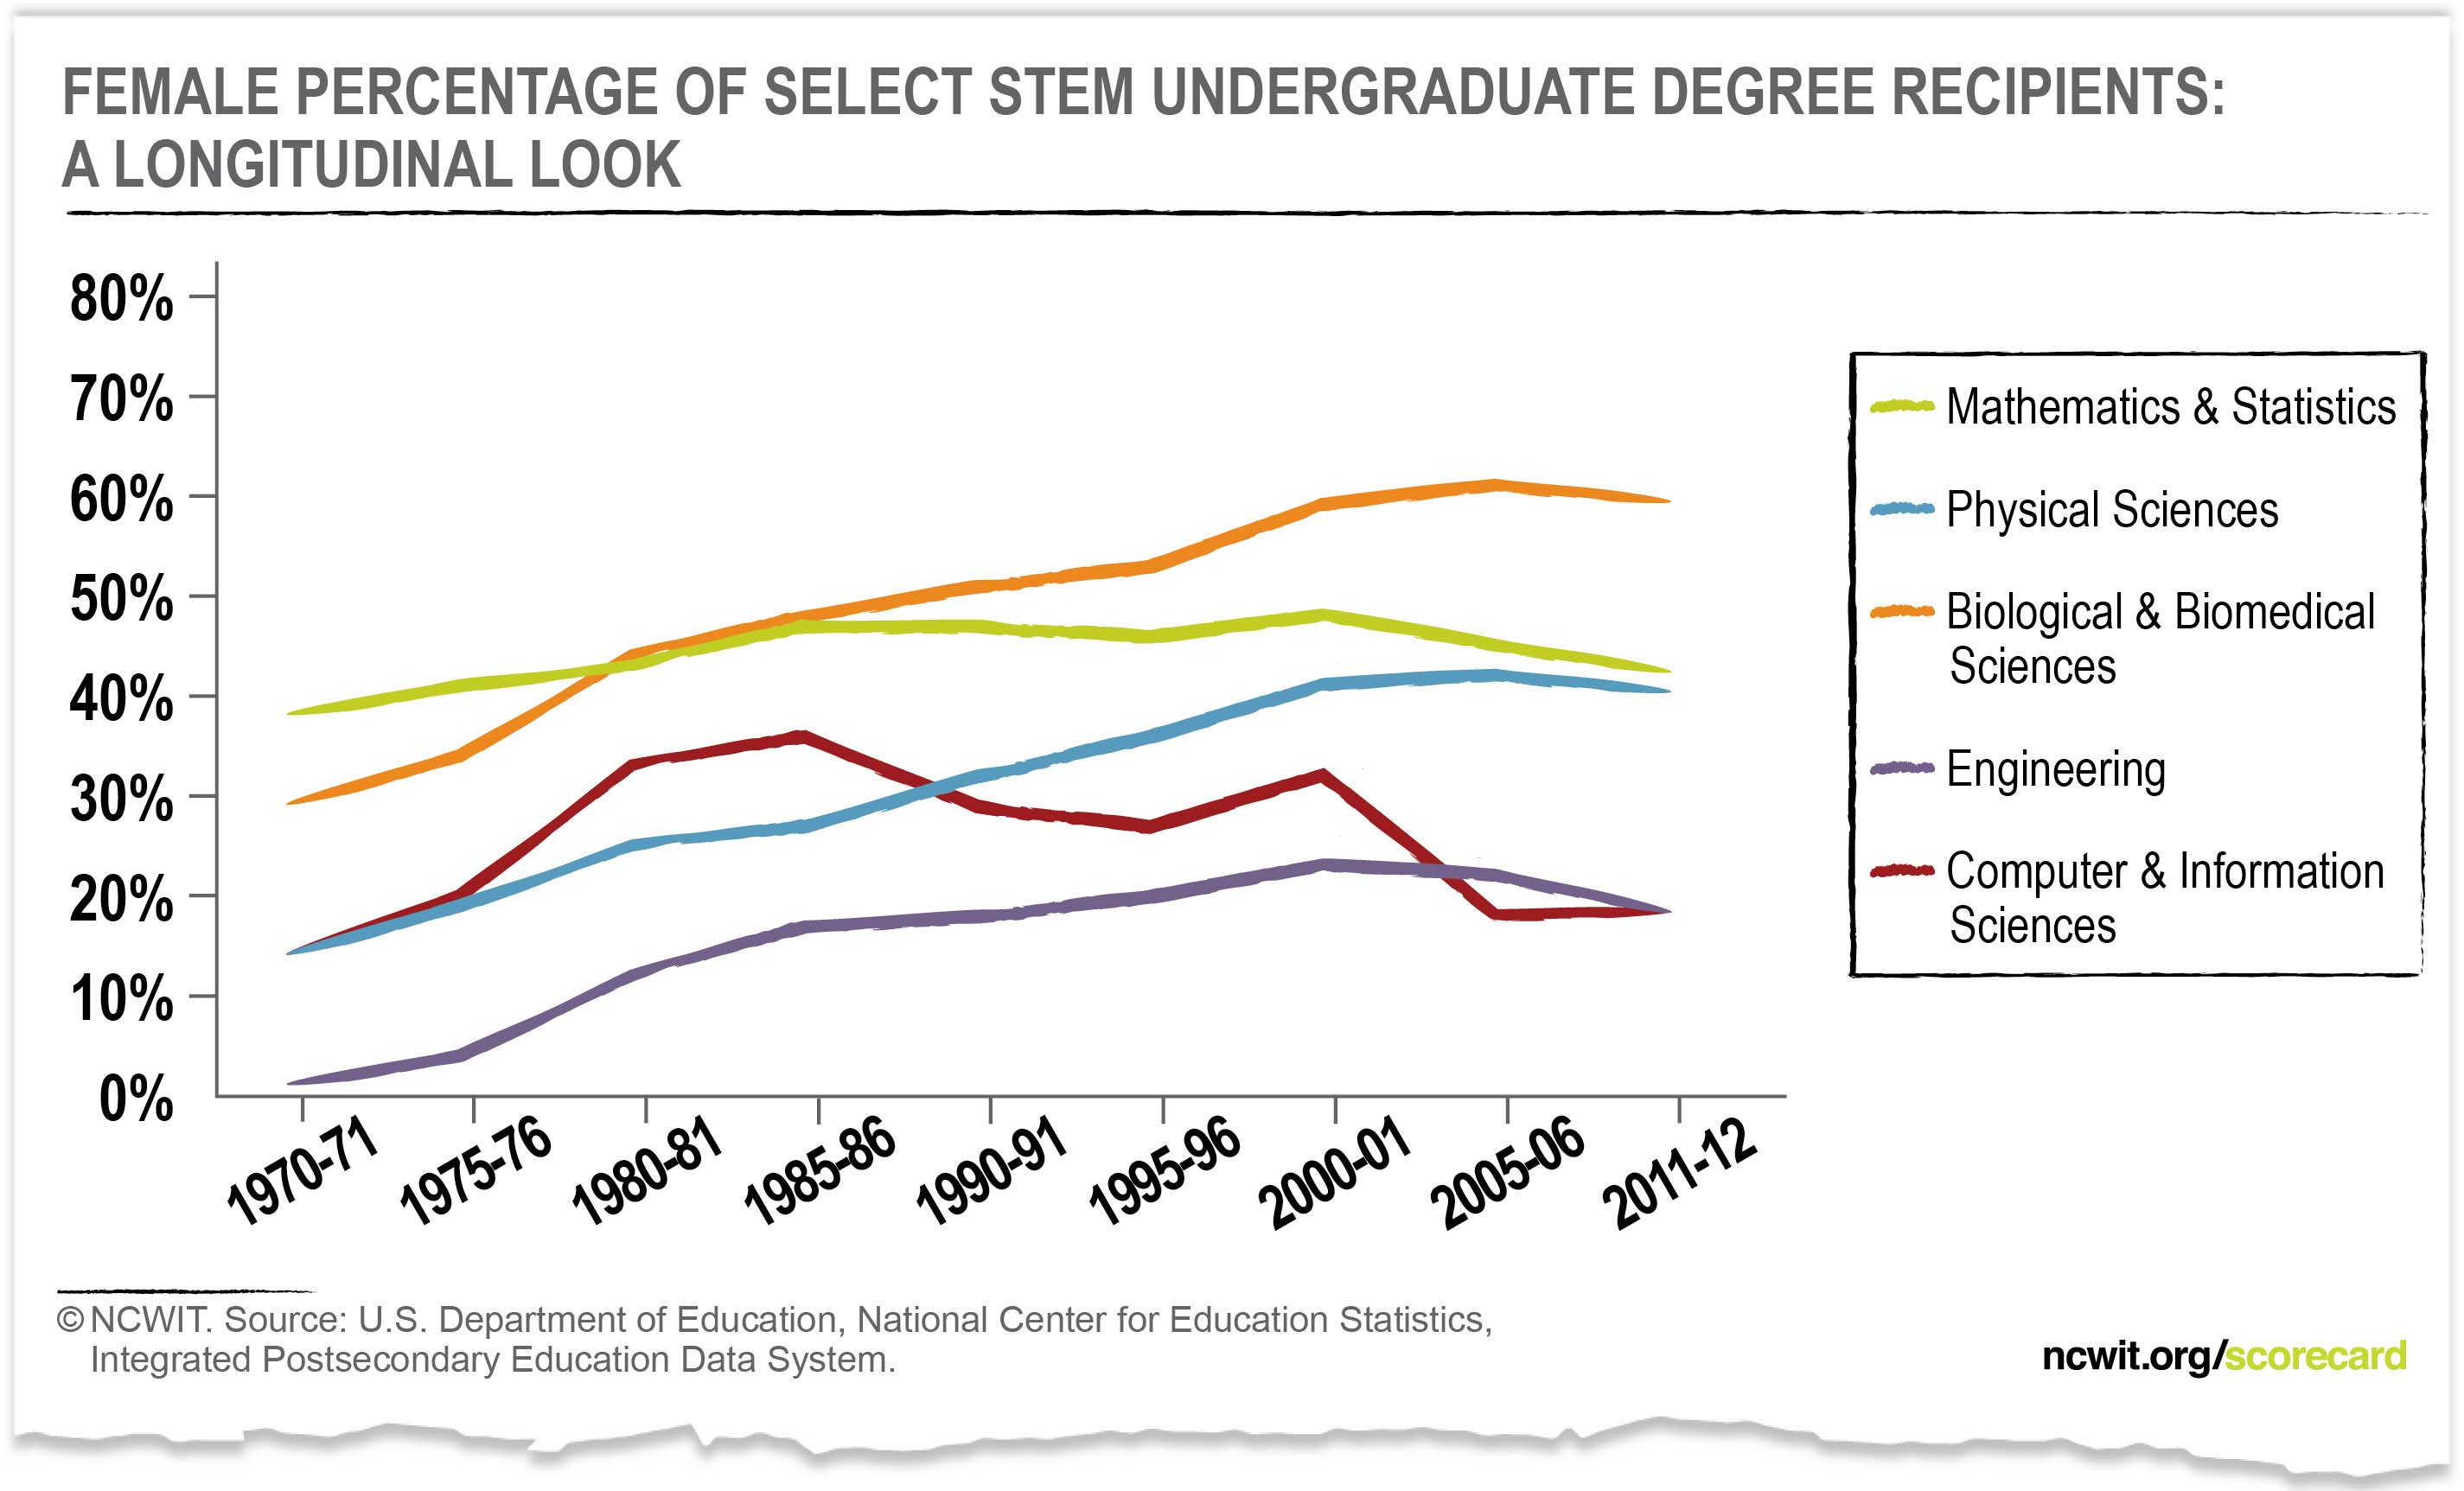
\includegraphics[width=0.7\textwidth]{percentwomencs}
   \caption{Female Percentage of Select STEM Undergraduate Degree Recipients}
   \label{femSTEMgrad}
\end{figure}

\begin{figure}[hbtp]
  \centering
  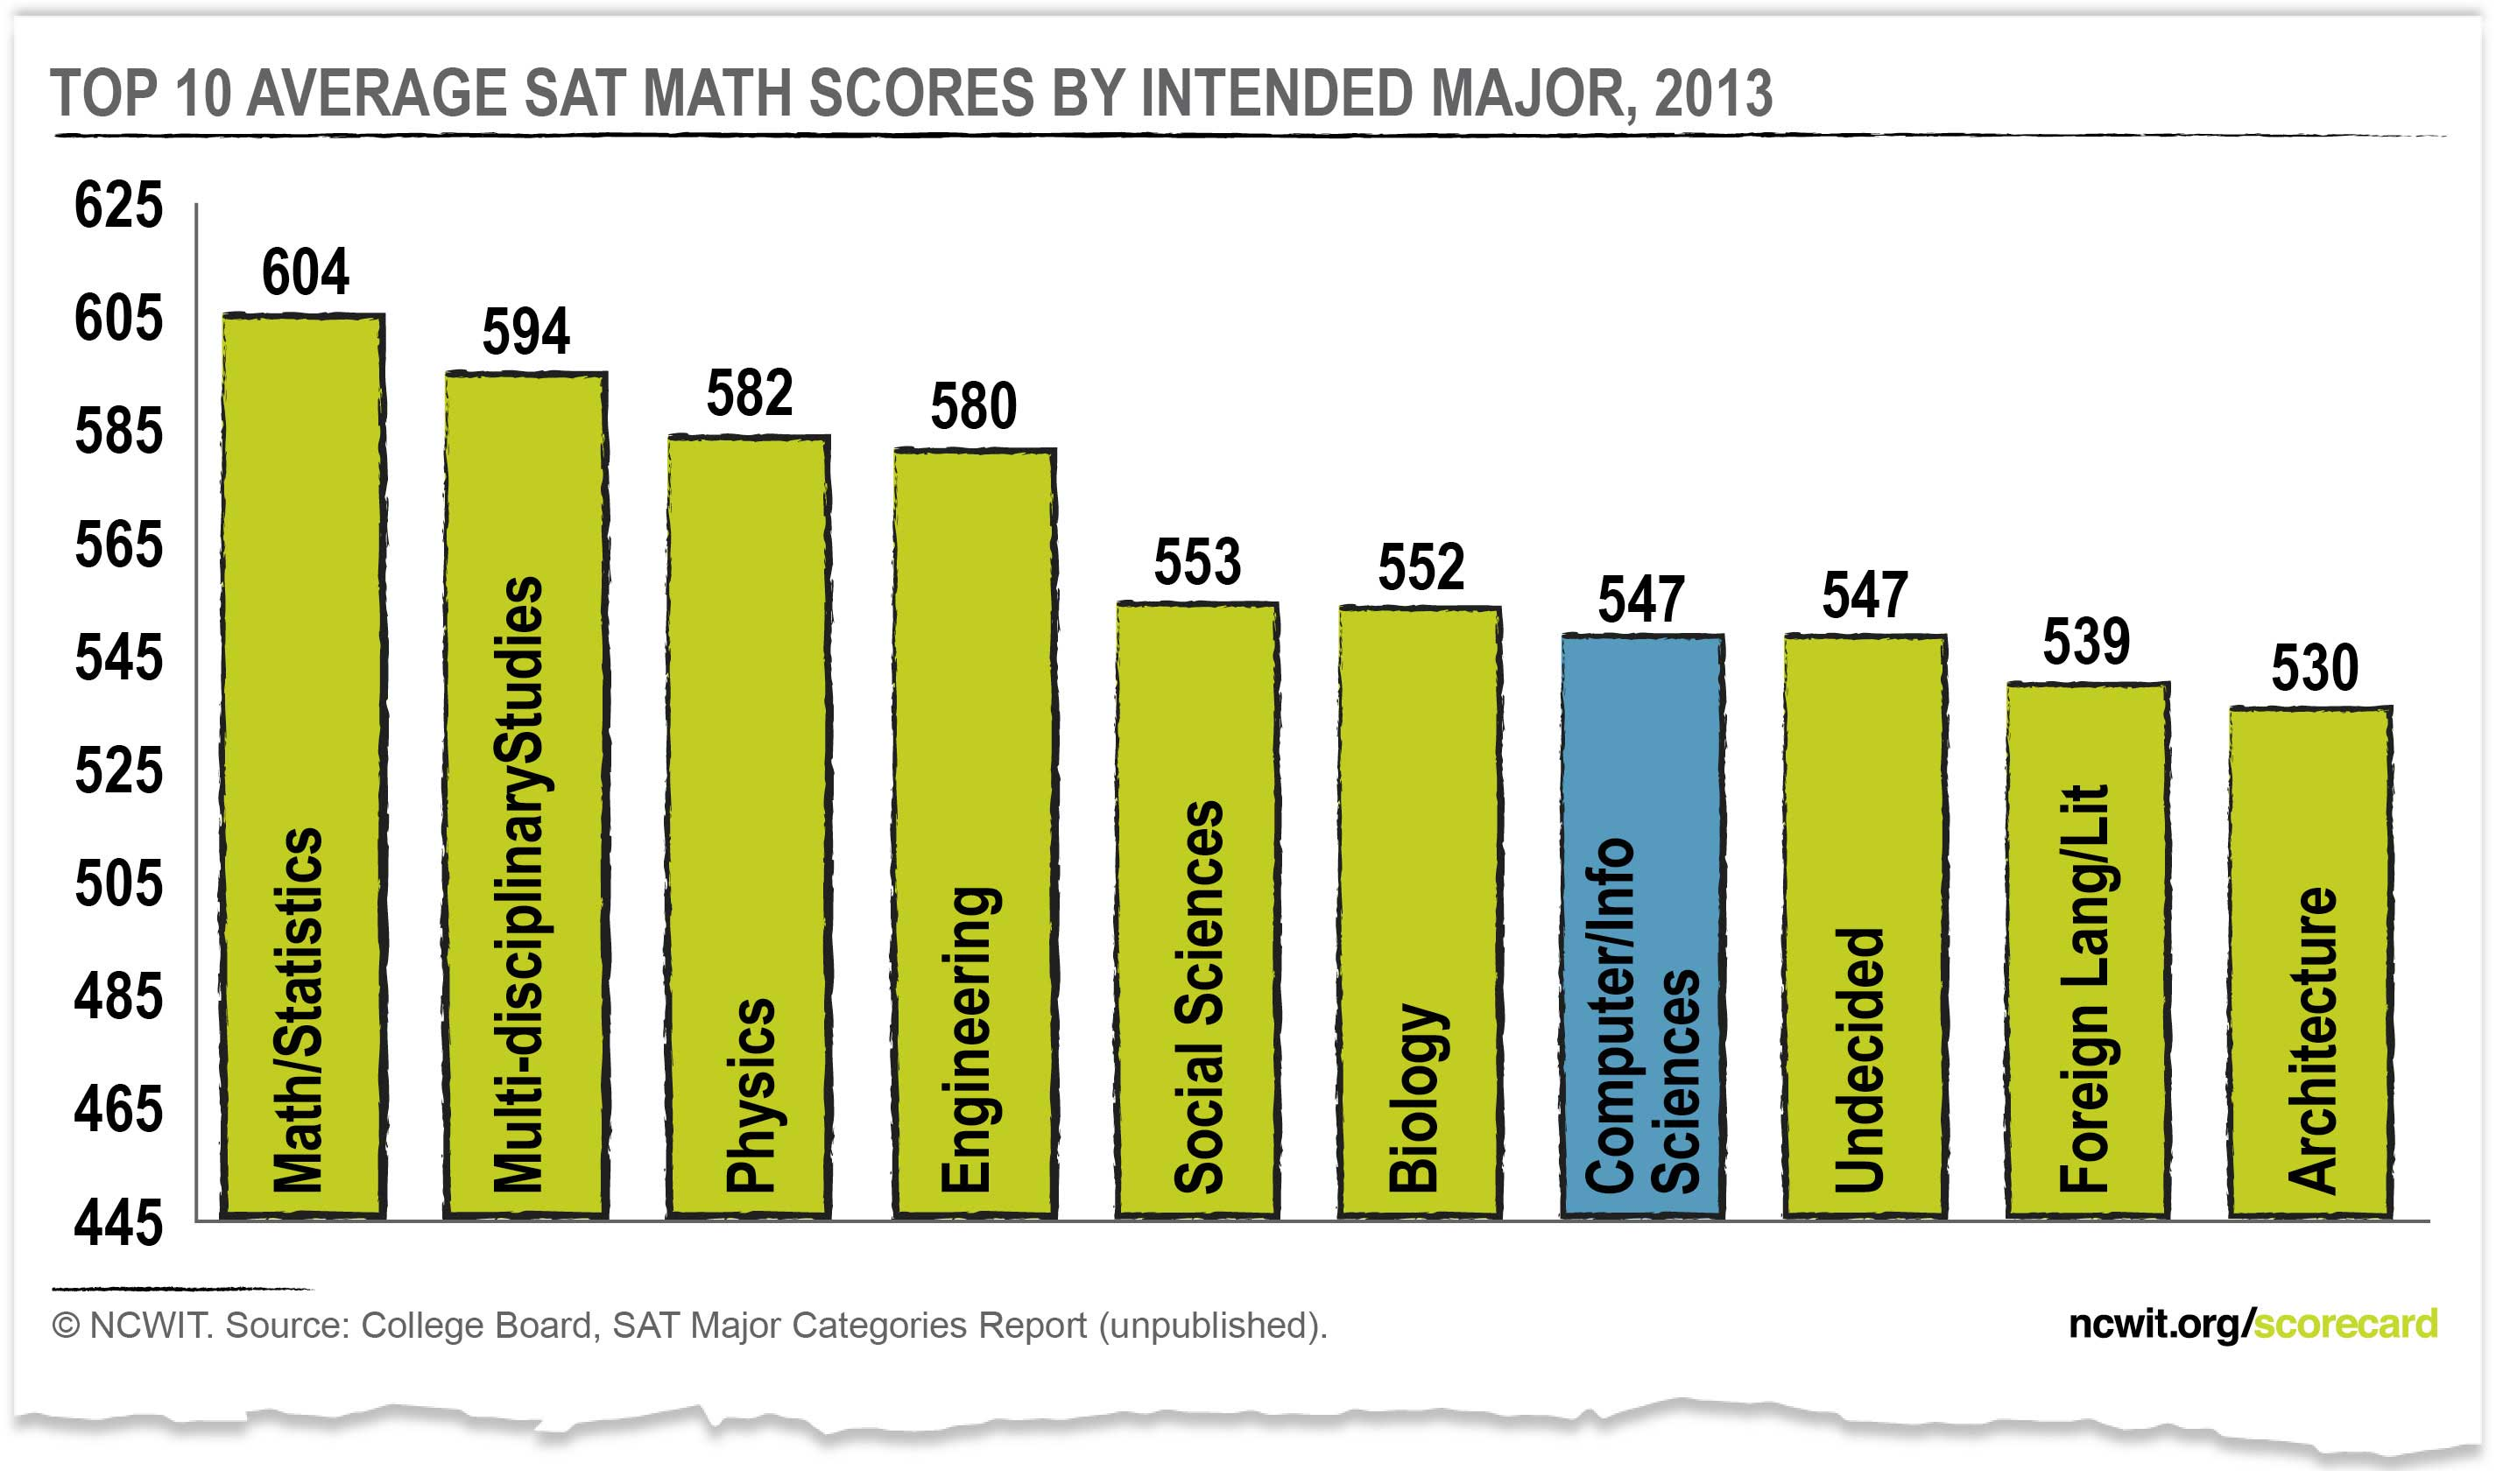
\includegraphics[width=0.7\textwidth]{TopSATMathIntendedMajor2013_NCWIT_SecondaryEd}
   \caption{Top 10 Average SATMathematics Scores by Intended Major}
   \label{satMathMajor}
\end{figure}

This issue of underrepresentation in CS is not only pertinent to CS education, but is also of direct importance to the health of the national economy. According to data from the U.S. Bureau of Labor Statistics, for every 150,000 computing jobs available, as a nation, we produce roughly 55,000 computing graduates to fill those jobs \cite{Labor-Statistics-BLS:aa}. Furthermore, the Bureau has projections which show that 51\% of the 9.2 million STEM (Science, Technology, Engineering and Mathematics) jobs between the years 2010 to 2020 will be in computing. Since 70\% of the population is underrepresented in computing, this makes the issue of equalizing participation in CS education a national issue. 

Figure \ref{popuGenderRace} shows the ethnic breakdown of the population along gender lines. From Figure \ref{popuCSUndergrad}, we can see that as of 2010, less than 20\% of CS degrees are obtained by women; to achieve parity this should be 50\%. Similarly, less than 20\% of CS degrees are obtained by underrepresented minorities; to achieve parity this should be 28\%. Underrepresented minority men are almost at parity in the attainment of undergraduate CS degrees as of 2010. 

\begin{figure}[hbtp]
  \centering
  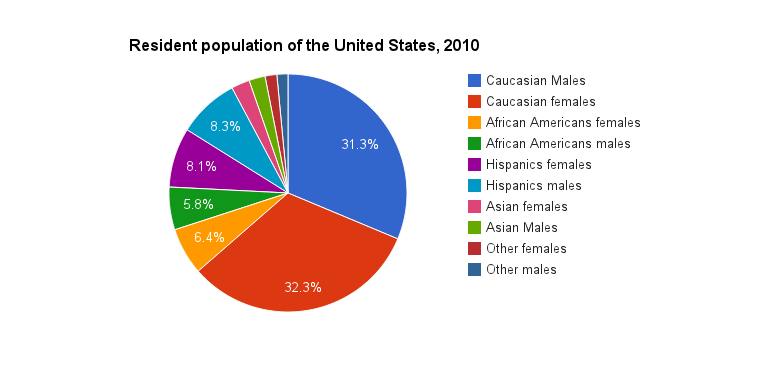
\includegraphics[width=1\textwidth]{chart_3}
  \caption{United States Census by Gender and Race, 2010}
  \label{popuGenderRace}
\end{figure}

\begin{figure}[hbtp]
  \centering
  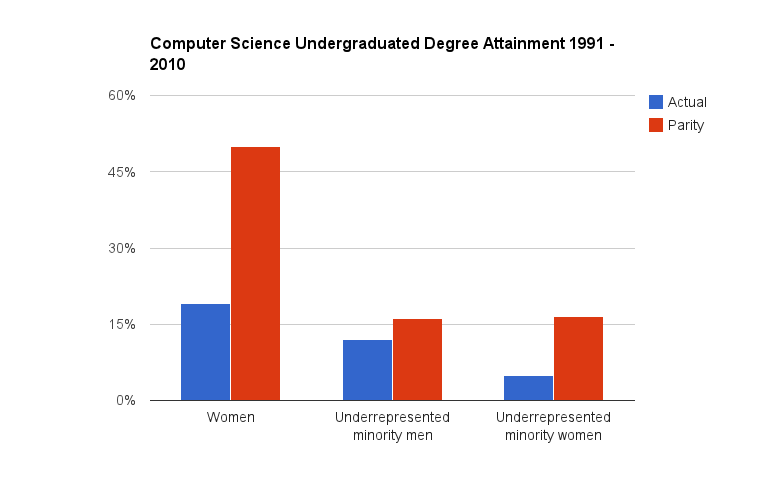
\includegraphics[width=1\textwidth]{chart_1}
   \caption{Undergraduate CS Degree Earned, 1991-2010}
  \label{popuCSUndergrad}
\end{figure}

As a means to address the low numbers of CS instruction at the high school level as well as the under-production of CS degrees at the collegiate level, a new AP CS Principles course has been developed to broaden participation in computing. Instead of focusing mostly on programming and algorithms, this new curriculum 
\begin{quote}
``introduces students to the central ideas of computing and computer science, to instill ideas and practices of computational thinking, and to have students engage in activities that show how computing and computer science change the world.'' \cite{Board:zr}
\end{quote}

UC Berkeley has been chosen as one of the pilot sites for this course \cite{Astrachan:2011:CPP:1953163.1953281}. The course with the title ``Beauty and Joy of Computing (BJC),'' is implemented in UC Berkeley's ``exploratory'' series as CS10---a CS course designed for non-majors. 

CS10 was specifically designed for non-majors to broaden participation. Since its inception, the course has been phenomenally successful in attracting female students, with the spring 2013 offering breaking the 50\% female barrier\footnote{ It is important to note, this is the first CS course, since UC Berkeley has been tracking student course data, that has ever achieved that feat.}. One of the goals of this work is to see if CS10 is able to serve as a successful gateway into the major, and more important, if a significant portion of the female students feel a strong sense of CS belonging.

\subsection *{Cognitive Perspective}

This work draws from the cognitive perspective on learning, emphasizing the understanding of concepts, of reasoning, and how they influences problem solving \cite{Greeno1996}, with particular emphasis on constructionism \cite{Papert1980}. A lot of the ideas for this research are motivated by the ideas that Seymour Papert touted in his seminal book \textit{Mindstorms: Children, Computers, and Powerful Ideas}. 

The most influential aspect of Papert's work is the idea that knowledge is built upon already existing ideas and schema that students have. The way we learn, Papert states is either by building upon our pre-existing theories, or creating new concepts, and then integrating them into our broader theories. Papert's idea that education should have cultural resonance is an idea that is fundamental to the creation of \textit{all} good curricula. In his book, \textit{Mindstorms}, Papert lays out how his love for gears was a great entry point and an intuitive cultural tool that he could use to understand formal systems. 
\begin{quote}
``In the Foreword of this book I described how gears helped mathematical ideas to enter my life. Several qualities contributed to their effectiveness. First they were a part of my natural ``landscape,'' embedded in the culture around me. \ldots Second, gears were part of the world of adults around me and through them I could relate to these people. Third, I could use my body to think about the gears. \ldots And finally, because, in a very real sense, the relationship between gears contains a great deal of mathematical information, I could use gears to think about formal systems.'' \cite[pp. 11]{Papert1980} 
\end{quote} 
These ideas that Papert lays down in this excerpt should be understood as the foundational articles upon which every culturally relevant pedagogical work should be built. Appropriating the turtle in the LOGO programming environment gave children a way to think about the principles of computation and the practice of programming. 


\section *{Design of an Inclusive CS0 Course}
At UC Berkeley, there are two separate ways a students can get a CS degree. They can either get a \emph{Bachelor of Arts (B.A.)} through the College of Letters and Sciences (L\&S), or get a \emph{Bachelor of Science (B.Sc.)} through the College of Engineering. The major difference between the two tracks is that students who get the B.A. get to take breadth requirements that gives them exposure to more of a liberal arts education. 

Once a student has decided that they might be interested in trying out CS, there are three major pathways the student can take. They can either take CS10, or CS 61A, or CS61AS---the self-paced version of CS 61A.

Having taking one of these classes, if a student then decides they are interested in either majoring/minoring in computing, whatever the track that student is in, they have to take the CS ``61 series.'' This series comprises of three classes:
\begin{itemize}
\item CS61A - Structure and Interpretation of Computer Programs.\\Introduction to programming and computer science. This course exposes students to techniques of abstraction at several levels: (a) within a programming language, using higher-order functions, manifest types, data-directed programming, and message-passing; (b) between programming languages, using functional and rule-based languages as examples. It also relates these techniques to the practical problems of implementation of languages and algorithms on a von Neumann machine. There are several significant programming projects.\footnote{Taken from the UC Berkeley \href{http://guide.berkeley.edu/courses/compsci/}{course catalog}}.
\item CS61B - Data Structures.\\Fundamental dynamic data structures, including linear lists, queues, trees, and other linked structures; arrays strings, and hash tables. Storage management. Elementary principles of software engineering. Abstract data types. Algorithms for sorting and searching. Introduction to the Java programming language. 
\item CS61C - Machine Structures.\\The internal organization and operation of digital computers. Machine architecture, support for high-level languages (logic, arithmetic, instruction sequencing) and operating systems (I/O, interrupts, memory management, process switching). Elements of computer logic design. Tradeoffs involved in fundamental architectural design decisions. 

\end{itemize}
Before the BJC curriculum was invented, the introductory course that was designed to serve non-majors was titled: ``Computer Science 3: Introduction to Symbolic Programming (CS3)''. The course was created to help students get ready to succeed in CS61A, the first CS class designed for majors. As a result, it used the same programming language that was used in CS61A, Scheme---a functional style, text-based language.

In her study of attrition in undergraduate CS at Berkeley, Lewis found that female students were disproportionately weeded out of the track, often starting at CS3 \cite{Lewis:EECS-2010-132}. For those students who had no prior programming background---majority female---CS3 served as a gateway to get them ready to succeed in the 61 series. The Lewis 2010 study used the CS3 online curriculum database to analyze the attrition patterns for 14 semesters, from the fall of 2002 to the spring of 2009. According to Lewis:
\begin{quote}
``When controlling for level in school, major and the semester and year the course was taken, the odds of a female student dropping the course is 32.0\% higher than for a male student.''\cite{Lewis:EECS-2010-132}
\end{quote}
Over her 14 year span of the data, she found the drop-out rates for female students was 27\% while that of male students was 20\%. Further, she noted that certain semesters like Fall 2006, female students dropped out of the class by 46\% while only 18\% of their male counterparts dropped the class. Furthermore, she found when controlling for the level in school, the major, and the semester/year the course was taken; the odds of a female student dropping the course was 32.0\% higher than for a male student.

In the past, most introductory to CS curriculum took a narrow view and placed priority on teaching the skill of programming. There was not a lot of emphasis placed on motivation, or the impact of technology on society. CS3 curriculum adhered to that paradigm, it was devoid of computing in the context of society. A student taking the CS3 curriculum would not have the opportunity to connect their CS knowledge to the human beings that created the knowledge, to the conditions that enabled the creation of the knowledge, and to the implications of the knowledge. It was a sterile approach that chugged computation down the throats of the students. 

The BJC approach fundamentally deviates from that by placing computational knowledge as a tool that should be in service of society. In addition to learning about conditionals, recursion, higher-order functions and so on, students are also introduced to contemporary issues at the intersection of CS and society. CS10 has been offered at UC Berkeley for Since 2010. In the 2010 pilot alone, 43 of the 77 college students chose to continue to the next more demanding first course intended for CS majors, CS61A.

\section *{Research Methods}

Formative, mixed-method research was conducted to test out the effectiveness of \emph{Beauty and Joy of Computing} (BJC) curriculum as implemented in UC Berkeley's CS10, in attracting historically underrepresented students. To gain a comprehensive analysis into the socio-curricular effectiveness of the BJC curriculum as the first class in a student's CS trajectory, it was benchmarked against CS61A---the first class for majors, and increasingly, for non-majors as well. 

Survey instruments were developed to measure participants' self-reported efficacy along several dimensions. To determine the role of identity and self efficacy; as well as the role of mentors in attracting underrepresented students, previously constructed instruments from \cite{Martin:2013fk} in their attitudinal study of CS in the Level Playing Field's Summer Math and Science Honors Academy (SMASH) were used. Additional instruments were developed by the researchers to measure cultural competency. The survey uses a 5-point Likert scale (where 1 = Not Really, 3 = Neutral and 5 = Absolutely).

Along with the surveys, interviews were conducted to get a deeper sense of the effectiveness of the BJC curriculum in attracting historically underrepresented students. These audio-recorded interviews were conducted at the university with participants that either attended CS10, CS61A, or both. Furthermore, participants were carefully chosen to reflect a broad spectrum of computing experiences from novice first time beginners to more advanced CS students. 

To gain a comprehensive analysis into the socio-curricular effectiveness of the BJC curriculum as the first class in a student's CS trajectory, it was benchmarked against CS61A---the first class for majors, and increasingly, for non-majors as well. The quantitative approach gave the opportunity to have a landscape view on the effectiveness of the curriculum in attracting the target audience, while the qualitative approach gave the opportunity to dig deeper into the specific lived experiences of the participants within the context of the classes under study. The research was constructed to answer the following research question: What impact does CS10 have in attracting female students into the major?


Survey instruments were developed to measure participants' interest along several dimensions as is shown in table \ref{SurveyInstrDim}. This was done by extending previously validated instruments. To measure students CS attitudes, previously constructed instruments from Titterton and Haynie were used \cite{Titterton2011}. To determine the role of identity and self efficacy; as well as the role of mentors in attracting underrepresented students, previously constructed instruments from \cite{Martin:2013fk} in their attitudinal study of CS in the Level Playing Field's Summer Math and Science Honors Academy (SMASH) were used. Additional instruments were developed by the researcher to measure cultural competency. The survey uses a 5-point Likert scale (where 1 = Not Really, 3 = Neutral and 5 = Absolutely). 
\begin{table}[!htbp]
  \begin{center}
    \begin{tabular}{ ll } 
    \multicolumn{2}{ c }%
    {\textbf{Dimensions Developed to Measure Participant's CS Interest}} \\[5pt] 
    \toprule
    Code & Dimension\\

    \midrule

    atcs & Attitudes about CS competency.\\ 
    atcsgender & Attitudes about the role of gender in CS\\
    atct & Understanding of computational thinking\\
    blg & Sense of belonging in the CS classroom.\\
    clet & Attitudes about social implications and ethics.\\
    cltrcmp & Understanding around cultural competency. \\
    mtr & Access to CS Mentors. \\
    prcs & Pre-Collegiate CS awareness. \\

    \bottomrule
    \end{tabular}
    \caption{Survey Instrument Dimensions to Measure CS Interest}
    \label{SurveyInstrDim}
  \end{center}
\end{table}



\subsection *{Qualitative Research: Interviews}
Along with the surveys, interviews were conducted to get a deeper sense of the effectiveness of the BJC curriculum in attracting historically underrepresented students. These audio-recorded interviews were conducted at the university with participants that either attended CS10, CS61A, or both. Furthermore, participants were carefully chosen to reflect a broad spectrum of computing experiences from novice first time beginners to more advanced CS students. 

Individual, semi-structured qualitative interviews ranging in 30-45 minute were conducted with participants. During these interviews, participants were asked about their use of computers, about their academic interest(s), their perception(s) of CS, their reason(s) for taking the class, and their experience around it. These interviews were taped and later transcribed. Analysis was guided by a grounded theory approach. Interview text was read first to identify emergent themes.


\section *{Location and Context}
There are three ways a student can take to become introduced to CS at UC Berkeley. The student may choose to take CS10, or chose to take CS61A, or instead choose to take CS61AS---The self-paced version of Structure and Interpretation of Computer Programs. For the purposes of understanding the experience of undergraduates students around introductory CS, the research context focused primarily on CS10 and CS61A.  

The two classes under evaluation to determine their effectiveness in broadening participation in computing are held every semester at the UC, Berkeley. CS10 has a class size of approximately 200+ students each semester, while CS61A has an approximate class size of 1000+ students. Participation in both classes are continuously growing at the university. As of the writing of this study, CS10 has a near 50-50 gender breakdown between male and female students, while CS61A's gender breakdown is approximately 34\% female and 66\% male.


\section *{Participants}

The participants that were part of this evaluation came from CS10 and CS61A. These were mostly undergraduates whose demographic skew strongly towards White and Asian students. Surveys were conducted with 882 participants, while interviews were done with 24 participants. Participants where recruited for the interviews based on their willingness to participate in the study from their responses to the surveys. Tables \ref{participants}, and \ref{interviewParticipants} show the breakdown of the participants in the study.
\begin{table}[!htbp]
  \begin{center}
    \begin{tabular}{ lll } 
    \multicolumn{3}{ c }%
    {\textbf{Survey Participant Break Down}} \\[5pt] 
    \toprule
    Class & Female & Male \\[2pt]
    \midrule
    
    CS10 Fall 2014 & 144 & 116 \\
    CS10 Spring 2015 & 73 & 54 \\ 

    CS61A & 171 & 324 \\ 
    \midrule 

    Total & 388 & 494 \\ 
    \bottomrule
    \end{tabular}
    \caption{Survey Participants}
    \label{participants}
  \end{center}
\end{table}

In total, 170 male students, and 217 female students consented to participate in the research from CS10, while 324 male students, and 171 female students consented to participate in the research from CS61A. 

In order to test for statistically significance, a non-parametric alternative to the standard \textit{t} test, the Mann-Whitney \textit{U} test was used \cite{Mann1947}. This decision was made because the study generated ordinal data through the use of a Likert scale, and no statements can be made with regards to the distribution of the data. Further, the Mann-Whitney test has been validated as acceptable when dealing with datasets for which there are unequal sample sizes. The significance threshold was set at 0.05.

The data was divided into sets as follows: Students who had previous pre-collegiate exposure to CS were separated from those that did not. This brought the sample size down from 882, to 480 for students without prior exposure to CS. The sample as distributed along gender and class as is shown in table \ref{StudentBreakDown}.

{\renewcommand{\arraystretch}{1.13}%
\begin{table}[h]
  \begin{center}
    \begin{tabular}{p{0.2\linewidth}llll} 

    \multicolumn{5}{ c }%
    {\textbf{Participants Breakdown For Analysis}} \\[5pt] 
    \toprule
    Class & Female & Male & Female & Male\\[2pt]
    & \multicolumn{2}{ c }{\textbf{With}}
    & \multicolumn{2}{ c }{\textbf{Without}}\\
    & \multicolumn{2}{ c }{Prior CS}
    & \multicolumn{2}{ c }{Prior CS}\\[5pt]
    \midrule
    
    
    CS10 & 45 & 48 & 85 & 101\\ 

    CS61A &  86 & 223 & 172 & 122 \\ 
    \midrule 

    Total & 131 & 271 & 257 & 223\\ 
    \bottomrule
    \end{tabular}
    \caption{Participants Broken Down by Prior Exposure to CS}
    \label{StudentBreakDown}
  \end{center}
\end{table}
}
The data was normalized to a range from 1 to 100. This decision was made to allow ease of interpretation in terms of percentages.

\section *{Results}
Table \ref{surveyfindingstable} shows the results of statistical test for significance---Using Mann Whitney Test---between the experience of students in CS10 and CS61A. Only survey instruments for whom p values were less than 0.05 where included in the table. These p-values indicate that there is a difference is the experience of CS10 students when compared to CS61A students.

As a result of the normalization of the data, the numbers denoting the responses of the students do not quite add up to 100. For the most part, they add up to 100 plus or minus 2, because of precision loss. 



\setlength{\extrarowheight}{1.5pt}
\begin{table}[!htbp]
\caption{Survey Finding with Statistical Significance} %title of the table
\centering % centering table
\begin{tabular}{|l|l|l||p{4cm}|l|} % creating eight columns
\hline\hline %inserting double-line
\multicolumn{2}{ |c| }{Groups} & Survey Instrument & P Value & Significance by Stars\\[0.5ex]
\hline % inserts single-line

CS10 & CS61A & atcs\_1 & 0.00000     & **** \\ \hline

CS10 & CS61A & atcs\_2 & 0.00011     & **** \\ \hline

CS10 & CS61A & atcs\_3 & 0.00424     & ** \\ \hline

CS10 & CS61A & atcs\_4 & 0.00000     & **** \\ \hline

CS10 & CS61A & atcs\_5 & 0.00035     & *** \\ \hline

CS10 & CS61A & atcs\_6 & 0.00001     & **** \\ \hline

CS10 & CS61A & atcs\_7 & 0.00000     & **** \\ \hline

CS10 & CS61A & atcs\_8 & 0.01949     & ** \\ \hline

CS10 & CS61A & atcs\_9 & 0.00004     & **** \\ \hline

CS10 & CS61A & atct\_5 & 0.00000     & **** \\ \hline

CS10 & CS61A & atct\_8 & 0.00000     & **** \\ \hline

CS10 & CS61A & atcsgender\_2 & 0.00913     & ** \\ \hline

CS10 & CS61A & blg\_3 & 0.00001     & **** \\ \hline

CS10 & CS61A & blg\_4  & 0.00000     & **** \\ \hline

CS10 & CS61A & clet\_2 & 0.00000     & **** \\ \hline


\end{tabular}
\label{surveyfindingstable}
\end{table}


\setlength{\extrarowheight}{1.5pt}
\begin{table}[!htbp]
\centering % centering table
\rotatebox{90}{ % rotate table
\begin{tabular}{|l|l|p{2cm}|p{1.5cm}|p{1.5cm}|p{2cm}|p{1.5cm}|p{2cm}|} % creating eight columns
\multicolumn{6}{c}%
      {Survey Finding with Statistical Significance [Data Disaggregated]
      (\textit{continued})}\\[5pt]
\hline\hline %inserting double-line
\multicolumn{2}{ |c| }{Groups} & Survey Instrument & Sample Group & P Value & Significance by Stars & P Value & Significance by Stars\\[1ex] 
\cline{5-8} 
\multicolumn{2}{|c|}{\textbf{}} & & &  \multicolumn{2}{c|}{\textbf{Prior CS}} & \multicolumn{2}{c|}{\textbf{NO Prior CS}}\\[0.5ex]
\hline % inserts single-line

CS10 & CS61A & atcs\_1  
& Class  & 0.02506  & * & & \\ \hline

CS10 & CS61A & atcs\_2 
&  Class  & 0.00448  & ** & & \\
& & &   Male  & 0.00883  & ** & & \\ \hline

CS10 & CS61A & atcs\_3 
& Class   &   0.01555   &   **    &   & \\
& & & Class   &   &   &   0.00895   & ** \\
& & & Female  &   &   &   0.00030   & *** \\ 
& & & Male    &   0.02903   & *   &   & \\ \hline

CS10 & CS61A & atcs\_4 
& Class   & 0.04441   & * & & \\
& & & Class  & & & 0.00341   & ** \\
& & & Male   & & & 0.00573   & ** \\ \hline

CS10 & CS61A & atcs\_6 
& Class  & 0.00638   & ** & & \\
& & & Male   & 0.00852   & ** & & \\ \hline

CS10 & CS61A & atcs\_7 
& Class  & 0.00064   & *** & & \\
& & & Male   & 0.02253   & * & & \\ \hline

CS10 & CS61A & atcs\_9
& Class  & 0.01197   & ** & & \\ \hline

CS10 & CS61A & atcsgender\_1
& Female  & & & 0.00214   & ** \\ \hline

CS10 & CS61A & atcsgender\_2 
& Class  & 0.01138   & ** & & \\ \hline

CS10 & CS61A & atct\_2
& Female & 0.02310   & *& & \\ \hline

CS10 & CS61A & atct\_3 
& Class   & & & 0.00911    & ** \\
& & & Female  & & & 0.00258    & ** \\ \hline
\end{tabular}}
\label{surveyDisAggregated}
\caption{Survey Finding with Statistical Significance [Data Disaggregated]} %title of the table
\end{table}

\setlength{\extrarowheight}{1.5pt}
\begin{table}[!htbp]
\centering % centering table
\rotatebox{90}{ % rotate table

\begin{tabular}{|l|l|p{2cm}|p{1.5cm}|p{1.5cm}|p{2cm}|p{1.5cm}|p{2cm}|} % creating eight columns
\multicolumn{6}{c}%
      {Survey Finding with Statistical Significance [Data Disaggregated]
      (\textit{continued})}\\[5pt]
\hline\hline %inserting double-line
\multicolumn{2}{ |c| }{Groups} & Survey Instrument & Sample Group & P Value & Significance by Stars & P Value & Significance by Stars\\[1ex] 
\cline{5-8} 
\multicolumn{2}{|c|}{\textbf{}} & & &  \multicolumn{2}{c|}{\textbf{Prior CS}} & \multicolumn{2}{c|}{\textbf{NO Prior CS}}\\[0.5ex]
\hline % inserts single-line
CS10 & CS61A & atct\_5
& Class & 0.00000   & **** & &  \\
& & & Class   & & & 0.00627 & ** \\
& & & Female   & 0.00024   & *** & & \\
& & & Male     & 0.00001   & **** & & \\ \hline

CS10 & CS61A & atct\_6
& Class  & 0.02987   & * & & \\ \hline
\end{tabular}}
\caption{Survey Finding with Statistical Significance [Data Disaggregated]} %title of the table
\end{table}


\setlength{\extrarowheight}{1.5pt}
\begin{table}[!htbp]
\centering % centering table
\rotatebox{90}{ % rotate table

\begin{tabular}{|l|l|p{1.5cm}|p{1.5cm}|p{1.5cm}|p{2cm}|p{1.5cm}|p{2cm}|} % creating eight columns
\multicolumn{6}{c}%
      {Survey Finding with Statistical Significance [Data Disaggregated]
      (\textit{continued})}\\[5pt]
\hline\hline %inserting double-line
\multicolumn{2}{ |c| }{Groups} & Survey Instrument & Sample Group & P Value & Significance by Stars & P Value & Significance by Stars\\[1ex] 
\cline{5-8} 
\multicolumn{2}{|c|}{\textbf{}} & & &  \multicolumn{2}{c|}{\textbf{Prior CS}} & \multicolumn{2}{c|}{\textbf{NO Prior CS}}\\[0.5ex]
\hline % inserts single-line

CS10 & CS61A & atct\_7 
& Class   & & & 0.03963 & * \\
& & & Female  & & & 0.04346 & * \\ \hline

CS10 & CS61A & atct\_8
& Class    & 0.00002   & **** & & \\
& & & Class  & & & 0.02489 & * \\
& & & Male     & 0.00268   & ** & & \\ \hline

CS10 & CS61A & blg\_1   
& Class   & & & 0.00023   & *** \\
& & & Female  & & & 0.00104   & *** \\
& & & Male    & & & 0.00755   & ** \\ \hline

CS10 & CS61A & blg\_2
& Class  & & & 0.00736   & ** \\
& & & Female & & & 0.01275   & ** \\ \hline

CS10 & CS61A & blg\_3
& Class   & 0.00393   & ** & & \\
& & & Class   & & & 0.00001   & **** \\
& & & Female  & 0.00024   & *** & & \\
& & & Female  & & & 0.00028   & *** \\
& & & Male    & & & 0.00050   & *** \\ \hline

CS10 & CS61A & blg\_4   
& Class  & 0.00716   & ** & & \\
& & & Class  & & & 0.00000   & **** \\
& & & Female & 0.00121   & *** & & \\
& & & Female & & & 0.00013   & **** \\
& & & Male   & & & 0.00002   & **** \\ \hline

\end{tabular}}
\label{surveyDisAggregatedCont}
\end{table}

\setlength{\extrarowheight}{1.5pt}
\begin{table}[!htbp]
\centering % centering table
\rotatebox{90}{ % rotate table

\begin{tabular}{|l|l|p{1.5cm}|p{1.5cm}|p{1.5cm}|p{2cm}|p{1.5cm}|p{2cm}|} % creating eight columns
\multicolumn{6}{c}%
      {Survey Finding with Statistical Significance [Data Disaggregated]
      (\textit{continued})}\\[5pt]
\hline\hline %inserting double-line
\multicolumn{2}{ |c| }{Groups} & Survey Instrument & Sample Group & P Value & Significance by Stars & P Value & Significance by Stars\\[1ex] 
\cline{5-8} 
\multicolumn{2}{|c|}{\textbf{}} & & &  \multicolumn{2}{c|}{\textbf{Prior CS}} & \multicolumn{2}{c|}{\textbf{NO Prior CS}}\\[0.5ex]
\hline % inserts single-line
CS10 & CS61A & clet\_2  
& Class   &   0.00246   &  **   &   & \\
& & & Class   &   &   &   0.00000 & **** \\
& & & Female  &   0.00490   &  **  &   & \\
& & & Female  &   &   &   0.00202  & ** \\
& & & Male    &   &   &   0.00013  & **** \\ \hline

CS10 & CS61A & cltrcmp\_2  
& Female  & 0.00804  & ** & & \\ \hline
\end{tabular}}
\end{table}


\clearpage
\section *{Findings}
\subsection *{On Belonging}

To investigate students' perception of CS fitness, as well as their sense of efficacy in the CS classroom, four instruments were designed and coded as follows: 
\begin{description} 
\item [blg\_1:] In this class, I feel I belong.
\item [blg\_2:] In this class, I feel awkward and out of place.
\item [blg\_3:] In this class, I feel like my ideas count.
\item [blg\_4:] In this class, I feel like I matter.
\end{description} 

Based on the data gathered from the survey, students generally had a stronger, statistically significant experience of belonging in CS10 as compared to CS61A, as can be seen in figure \ref{blg_Dim}. Nevertheless, it is important to notice that only around 50\% of female learners had a positive sense of belonging (\emph{p} = 0.00104) as can be seen from figure \ref{fig:blg_1_female_NO_CS}. 

When focusing on ideas, only about 50\% of female learners felt their ideas were important in the class (\emph{p} = 0.00028), as can be seen in figure \ref{fig:blg_3_female_NO_CS}. 

When asked about their sense of feeling important in the class, we observe a statistically significant (\emph{p} = 0.0000) difference between the experience of learners in CS10 versus their counterparts in CS61A, figure \ref{fig:blg_4}. 

Narrowing our analysis to the experience of learners \underline{without} prior exposure to CS, we see that for CS61A, similar proportions of learners of both gender feel like they don't matter, i.e., 35\% plus/minus 5. In contrast, only 10\% of boys (\emph{p} = 0.00002) felt unimportant versus 17\% of girls (\emph{p} = 0.00013) in CS10. Important to note is that when we look at female learners \underline{with} prior CS exposure, the proportion drops to 8\% (\emph{p} = 0.00121).

\begin{figure}[!htbp]
    \subfloat[]{%
    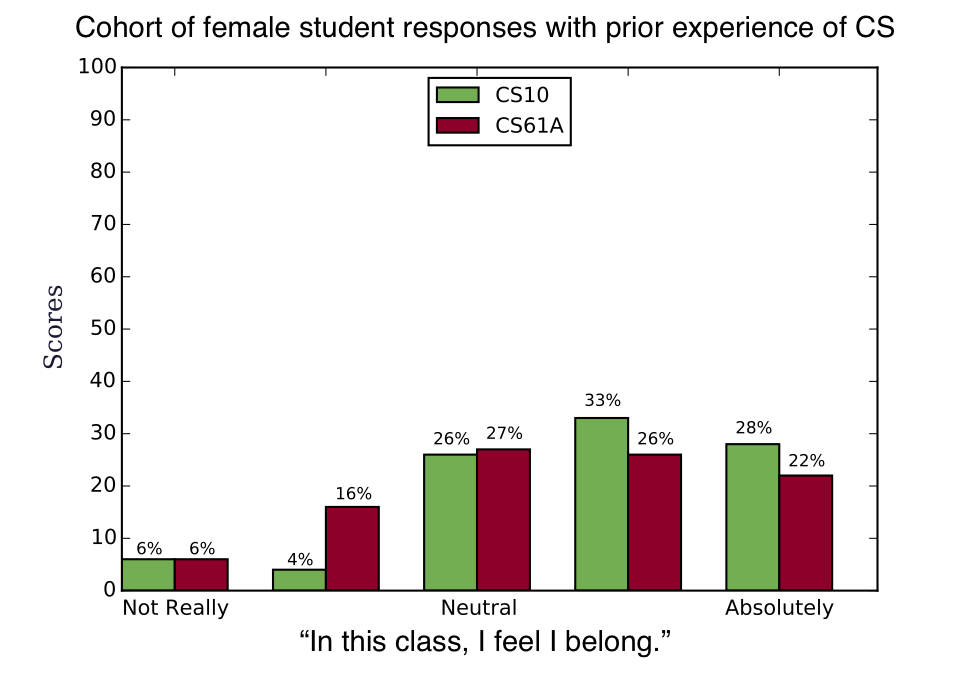
\includegraphics[width=0.5\textwidth]{figures/blg_1_female_CS.png}
    \label{fig:blg_1_female_CS}}
    \subfloat[]{%
    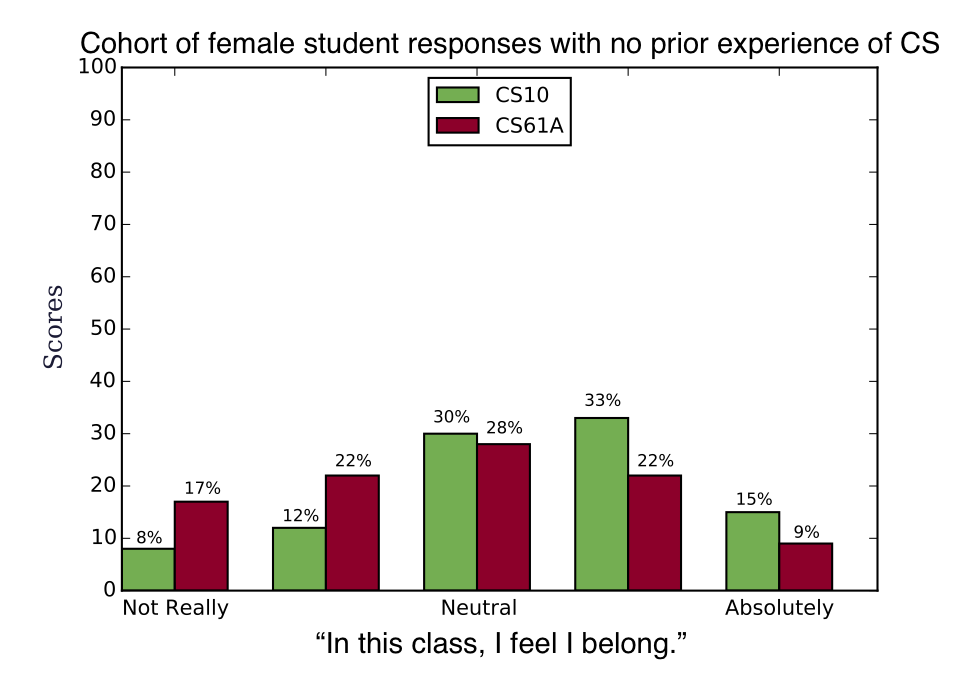
\includegraphics[width=0.5\textwidth]{figures/blg_1_female_NO_CS.png}
    \label{fig:blg_1_female_NO_CS}}
    \qquad
    \subfloat[]{%
    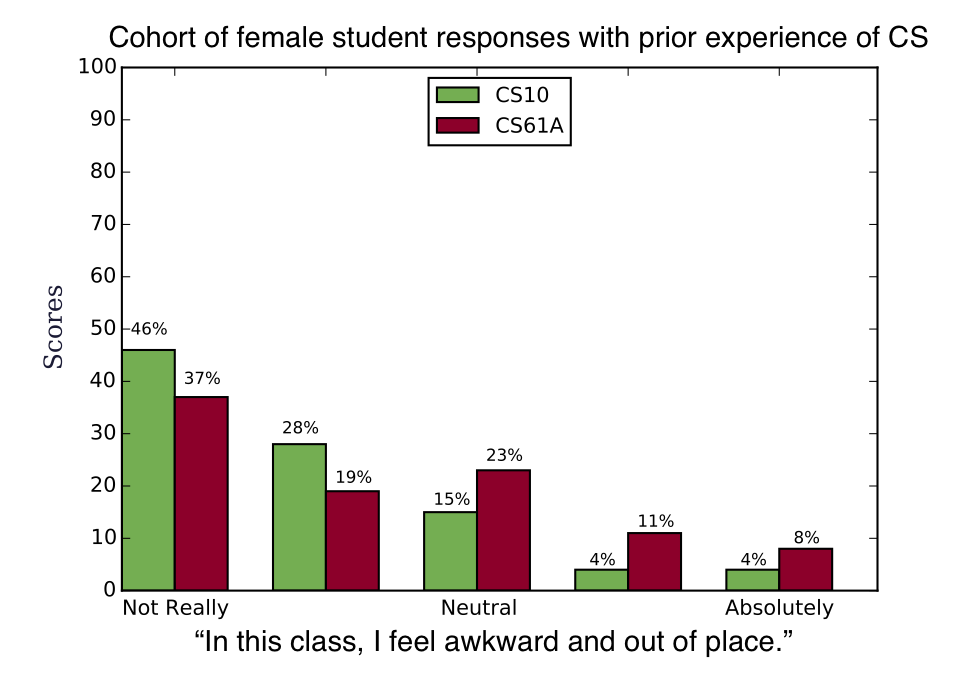
\includegraphics[width=0.5\textwidth]{figures/blg_2_female_CS.png}
    \label{fig:blg_2_female_CS}}
    \subfloat[]{%
    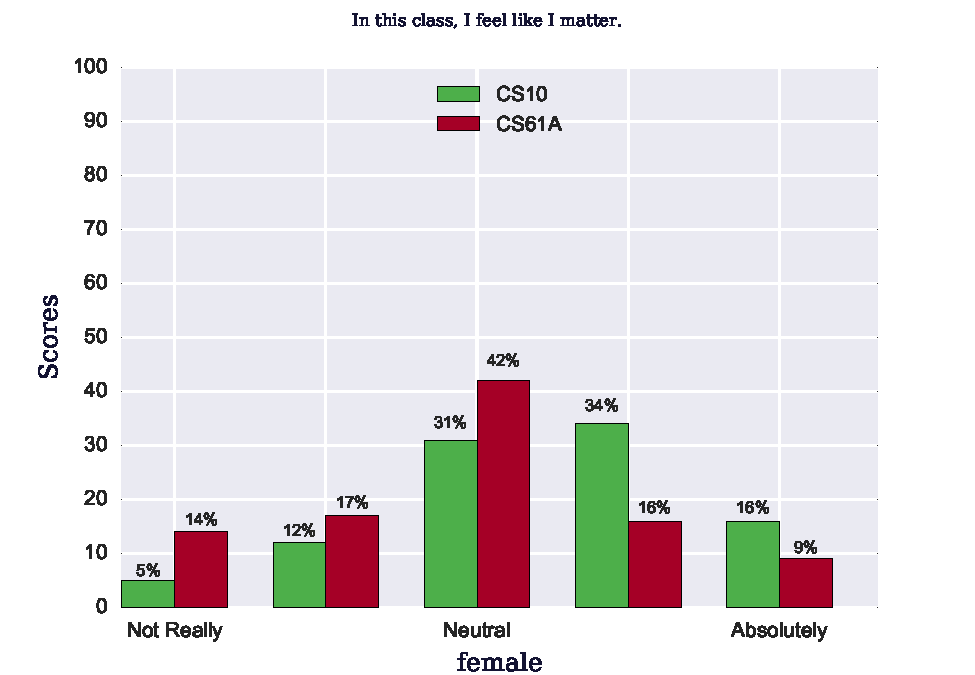
\includegraphics[width=0.5\textwidth]{figures/blg_2_female_NO_CS.png}
    \label{fig:blg_2_female_NO_CS}}
    \qquad
    \subfloat[]{%
    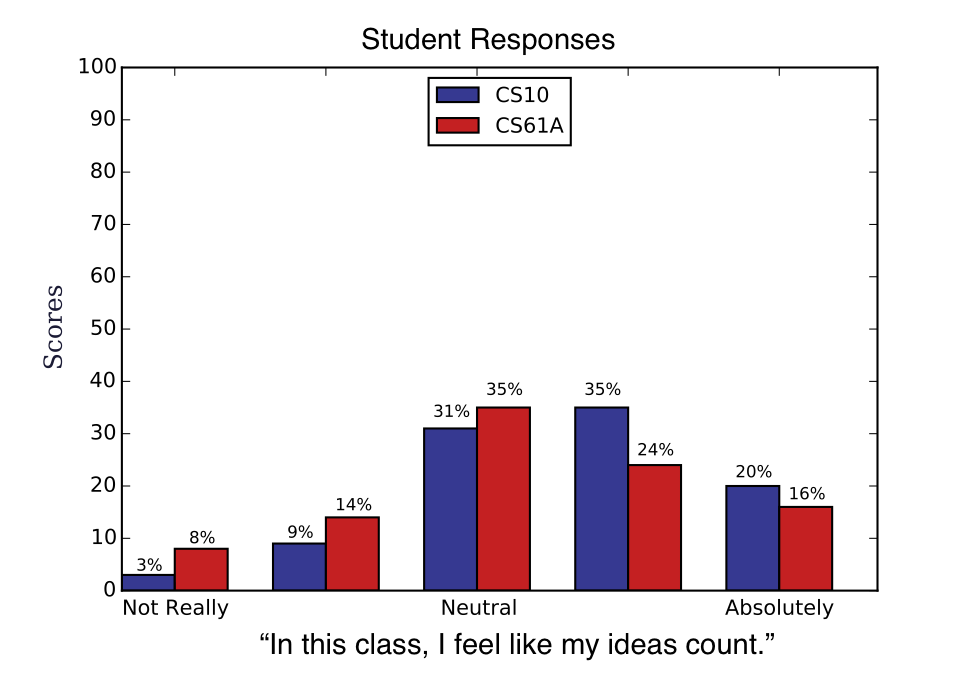
\includegraphics[width=0.5\textwidth]{figures/blg_3_CS61aVersusCS10.png}
    \label{fig:blg_3}}
    \subfloat[]{%
    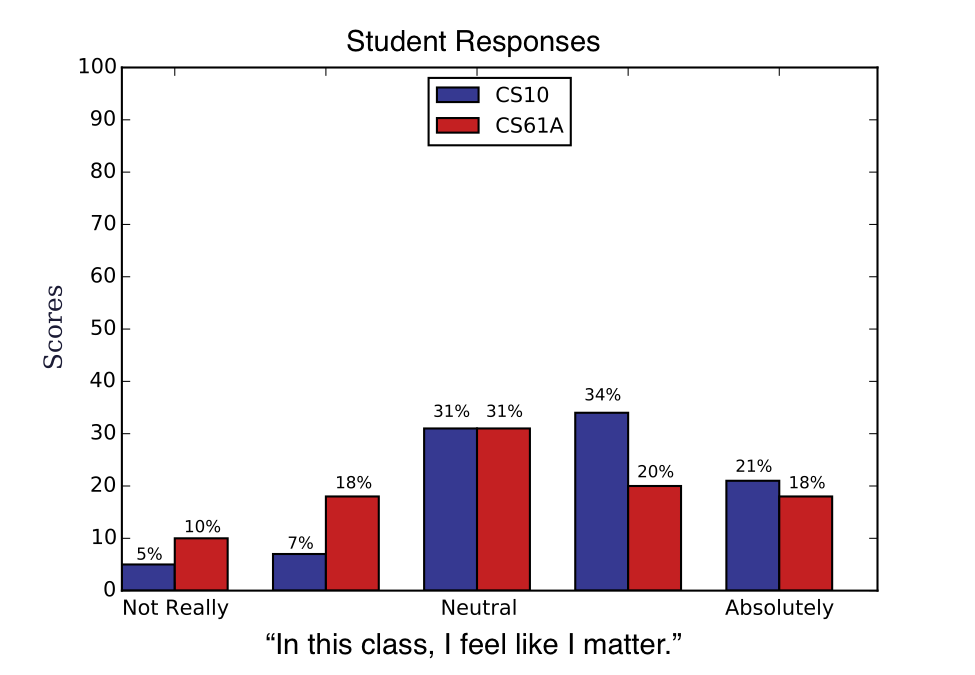
\includegraphics[width=0.5\textwidth]{figures/blg_4_CS61aVersusCS10.png}
    \label{fig:blg_4}}
  %
\caption{\textbf{Students' responses with regards to CS belonging.} \textit{Self reported responses are shown for four survey instruments. Sub-figures (a), (b), (c), and (d) show responses of female students disaggregated along two dimensions: \textbf{with} and \textbf{without} prior CS experience. From the data we can see that on average CS10 students have a better sense of belonging in intro CS at UC Berkeley.}}
\label{blg_Dim}
\end{figure}

%-------------------N O  P R I O R  C S  &  G E N D E R ---------------------%

\begin{figure}[!htbp]
  \centering
    \subfloat[]{%
    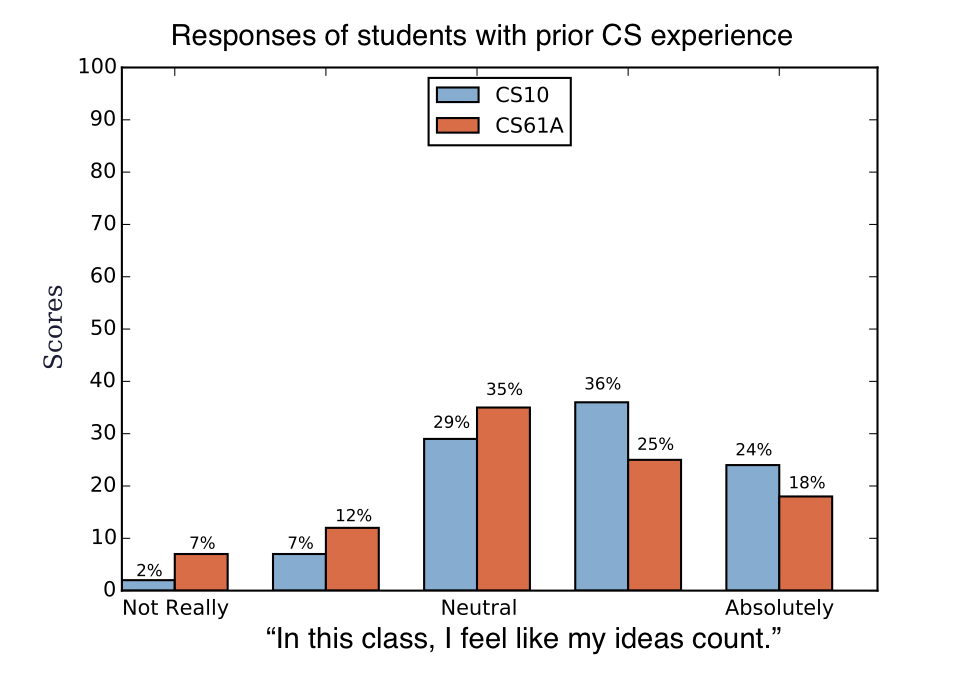
\includegraphics[width=0.5\textwidth]{figures/blg_3_CS61aVersusCS10_CS.png}
    \label{fig:blg_3_CS}}
    \subfloat[]{%
    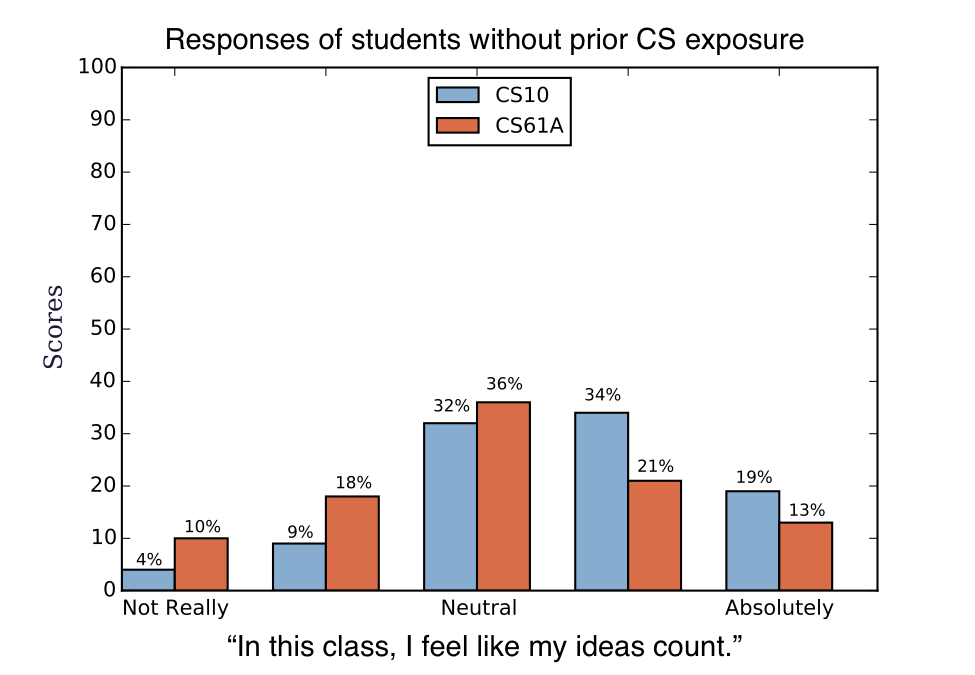
\includegraphics[width=0.5\textwidth]{figures/blg_3_CS61aVersusCS10_NO_CS.png}
    \label{fig:blg_3_NO_CS}}
    \qquad
    \subfloat[]{%
    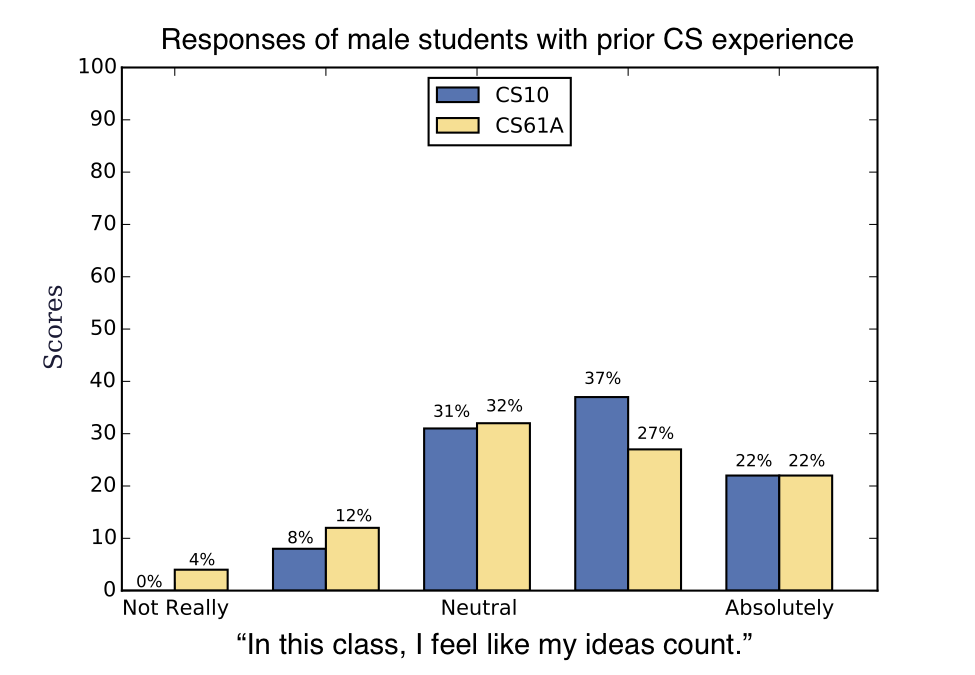
\includegraphics[width=0.5\textwidth]{figures/blg_3_male_CS.png}
    \label{fig:blg_3_male_CS}}
    \subfloat[]{%
    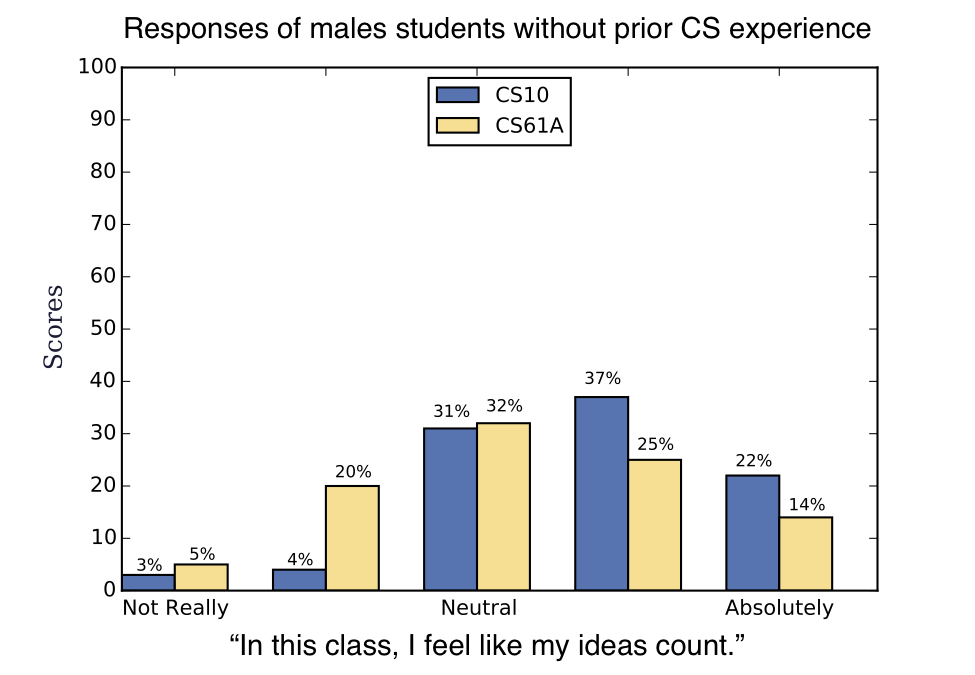
\includegraphics[width=0.5\textwidth]{figures/blg_3_male_NO_CS.png}
    \label{fig:blg_3_male_NO_CS}}
    \qquad
    \subfloat[]{%
    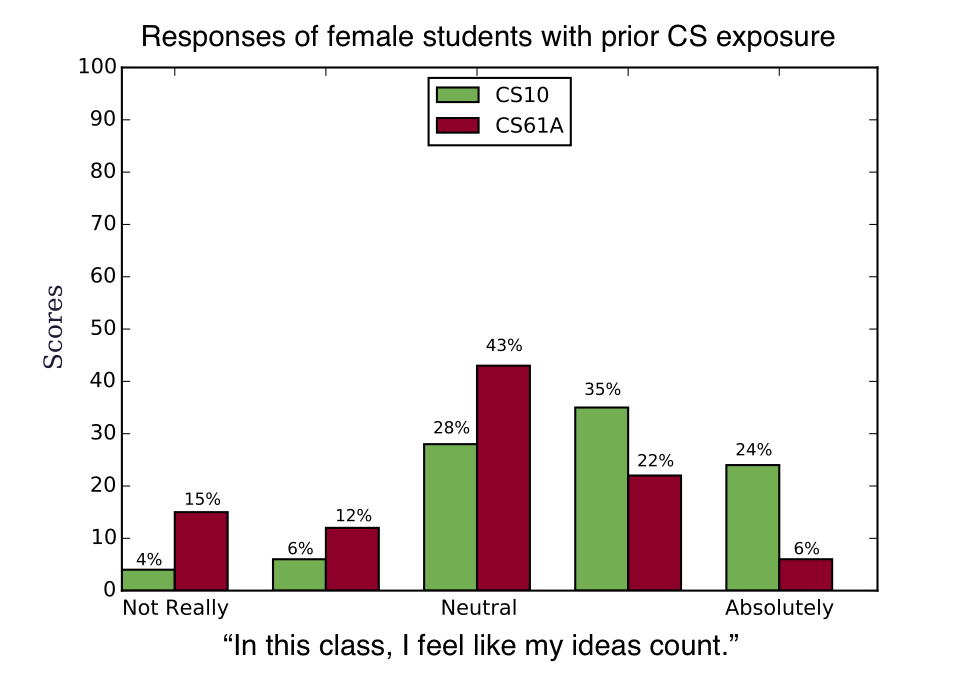
\includegraphics[width=0.5\textwidth]{figures/blg_3_female_CS.png}
    \label{fig:blg_3_female_CS}}
    \subfloat[]{%
    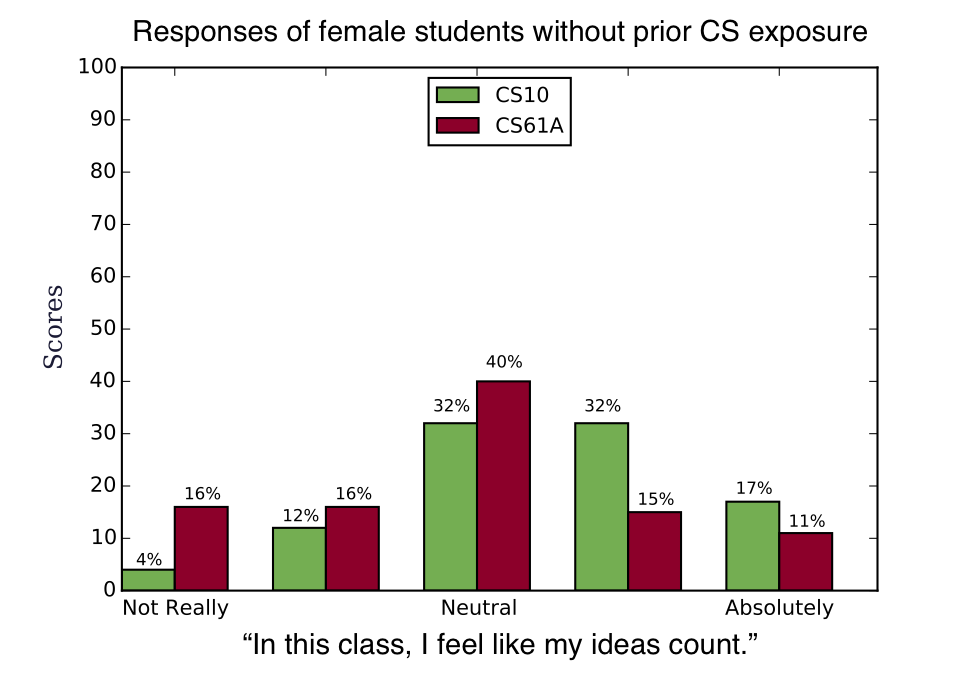
\includegraphics[width=0.5\textwidth]{figures/blg_3_female_NO_CS.png}
    \label{fig:blg_3_female_NO_CS}}
  %
\caption{\textbf{Students' responses for survey question: ``In this class, I feel like my ideas count."} \textit{Self reported responses are shown for the survey instrument. Sub-figures (a), and (b) show responses of students disaggregated along two dimensions: \textbf{with} and \textbf{without} prior CS experience. While sub-figure (b) through (f) show gendered responses, disaggregated along the same dimensions.}}
\label{blg_3_dis}
\end{figure}


%-------------------N O  P R I O R  C S  &  G E N D E R ---------------------%

\begin{figure}[!htbp]
  \centering
    \subfloat[]{%
    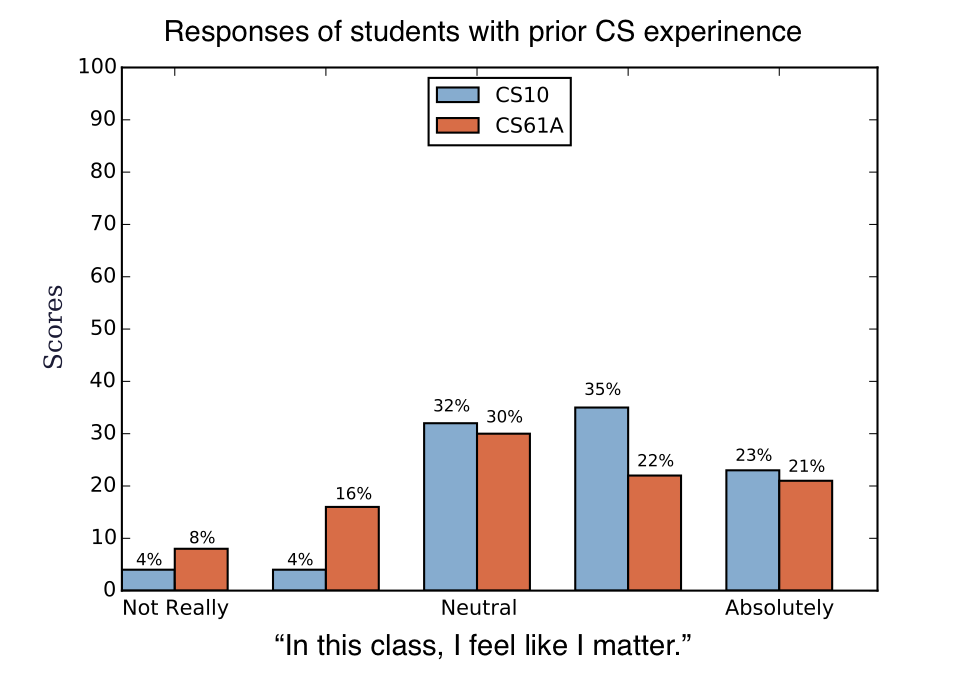
\includegraphics[width=0.5\textwidth]{figures/blg_4_CS61aVersusCS10_CS.png}
    \label{fig:blg_4_CS}}
    \subfloat[]{%
    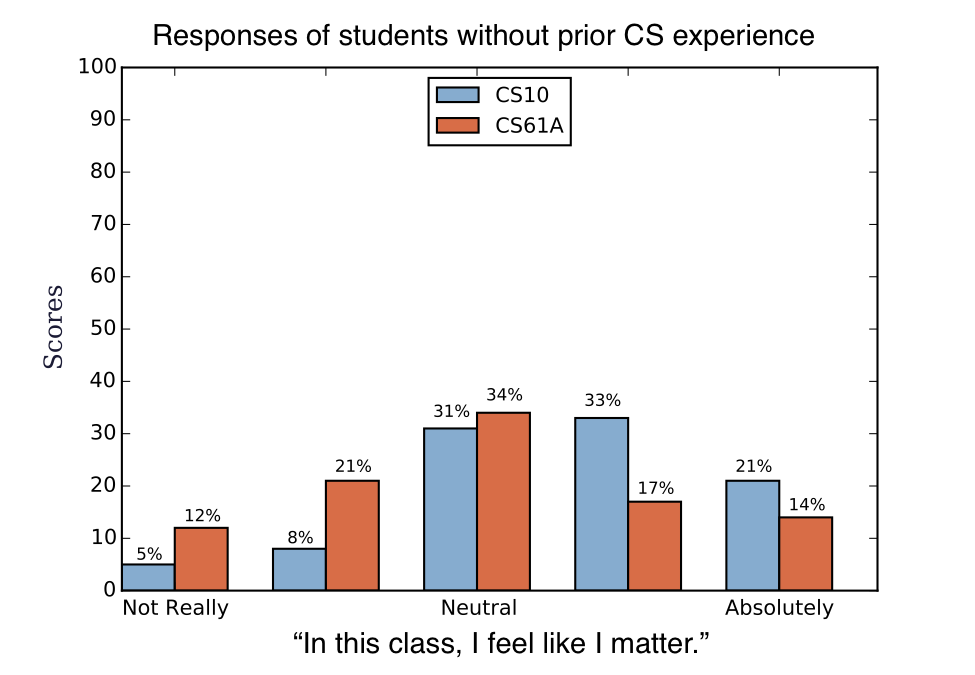
\includegraphics[width=0.5\textwidth]{figures/blg_4_CS61aVersusCS10_NO_CS.png}
    \label{fig:blg_4_NO_CS}}
    \qquad
    \subfloat[]{%
    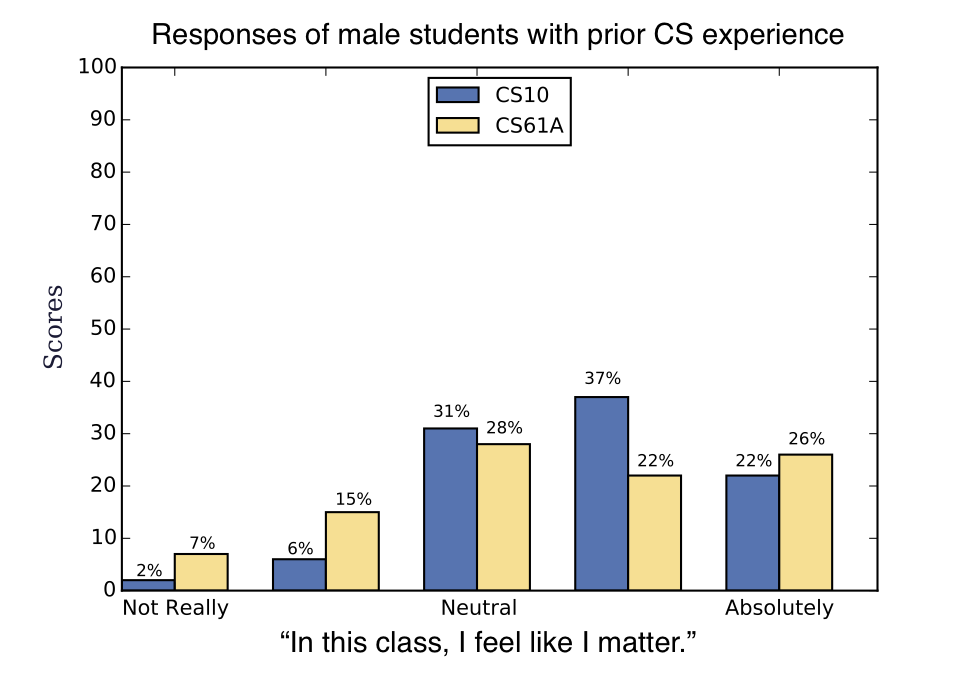
\includegraphics[width=0.5\textwidth]{figures/blg_4_male_CS.png}
    \label{fig:blg_4_male_CS}}
    \subfloat[]{%
    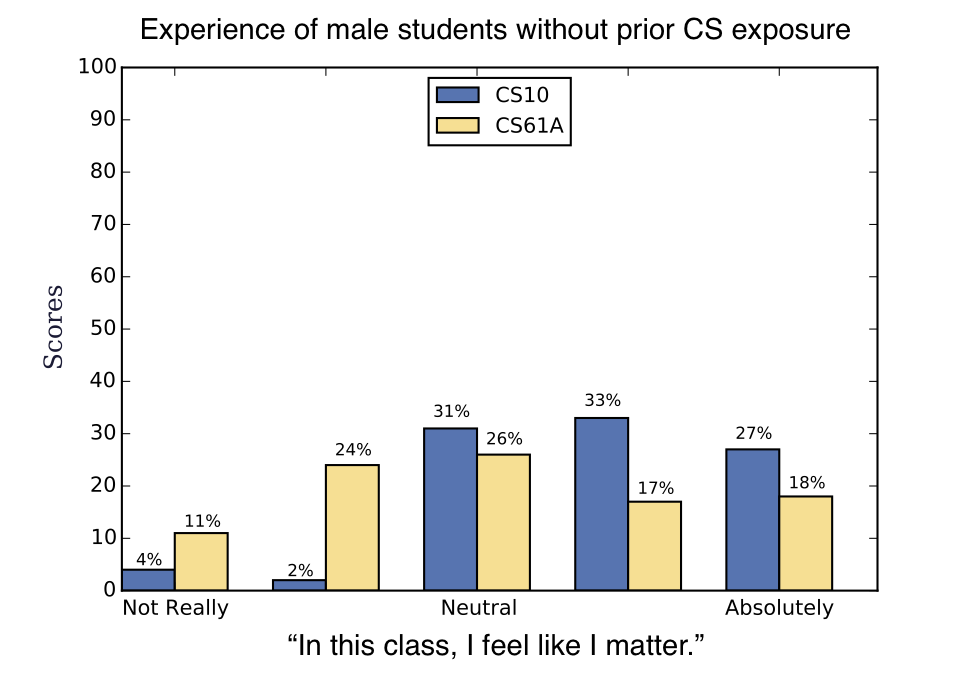
\includegraphics[width=0.5\textwidth]{figures/blg_4_male_NO_CS.png}
    \label{fig:blg_4_male_NO_CS}}
    \qquad
    \subfloat[]{%
    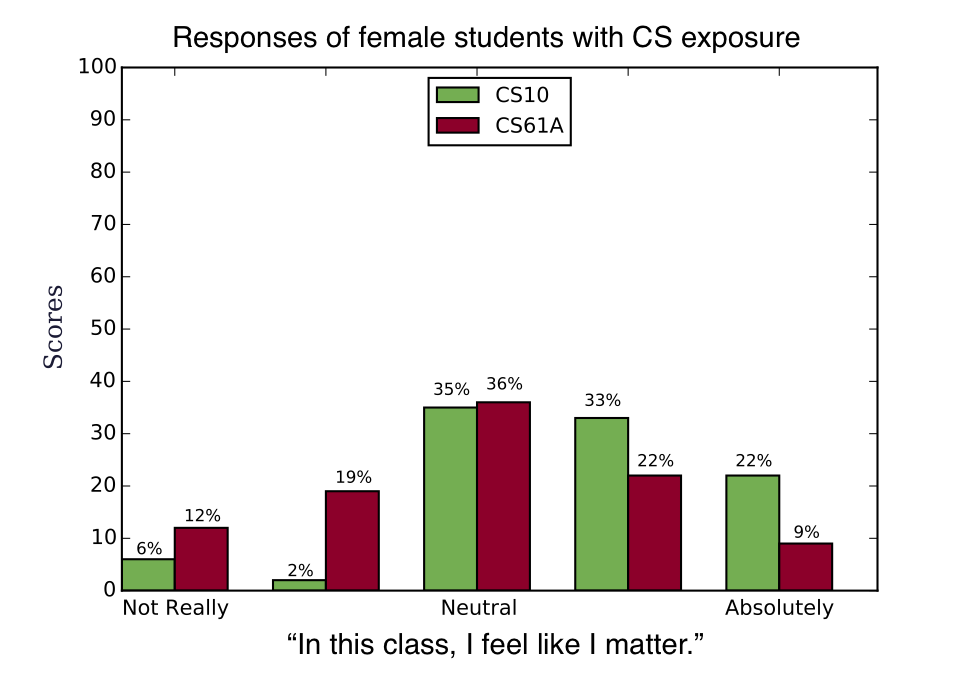
\includegraphics[width=0.5\textwidth]{figures/blg_4_female_CS.png}
    \label{fig:blg_4_female_CS}}
    \subfloat[]{%
    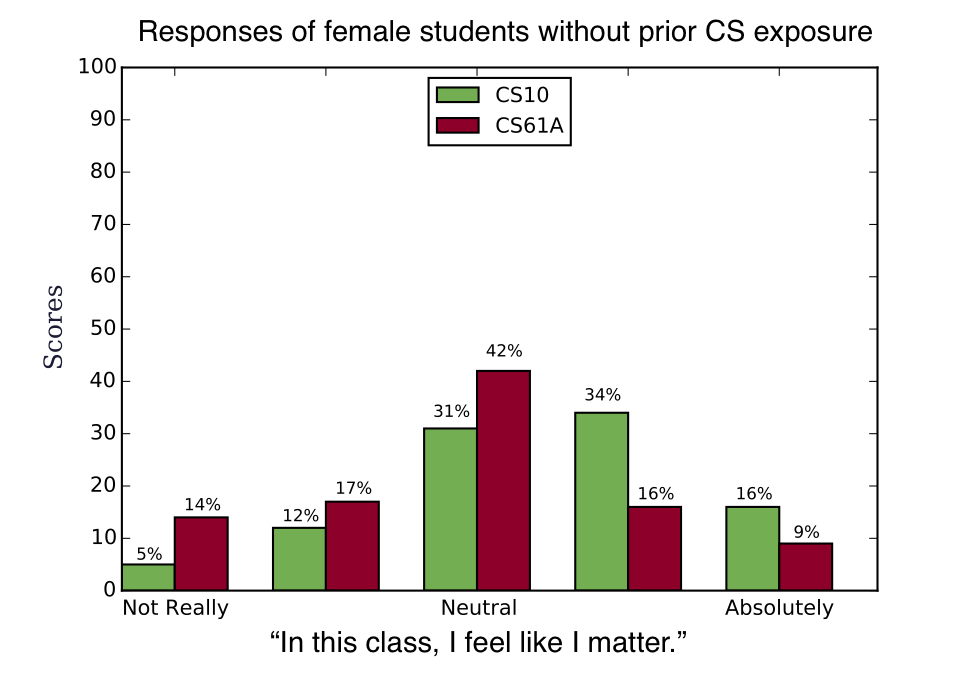
\includegraphics[width=0.5\textwidth]{figures/blg_4_female_NO_CS.png}
    \label{fig:blg_4_female_NO_CS}}
  %
\caption{\textbf{Students' responses for survey question: ``In this class, I feel like I matter.''} \textit{Self reported responses are shown for the survey instrument. Sub-figures (a), and (b) show responses of students disaggregated along two dimensions: \textbf{with} and \textbf{without} prior CS experience. While sub-figure (b) through (f) show gendered responses, disaggregated along the same dimensions.}}
\label{blg_4_dis}
\end{figure}


\subsubsection *{Effect of CS10 on CS61A Experience: Belonging}
First, let's take a gendered look at learners self-reported belonging. From figure \ref{blg_1_male_female}, we observe that 51\% of female learners have positive sense of belonging versus 61\% of male learners.

To see what effect participation in CS10 has on students' sense of belonging in CS61A, a data subset was created of CS61A students who had previously taken CS10. This new subset had a sample size N=40, with 18 female subjects and 22 male subjects.

Looking to see if the experience of CS10 increased female students sense of belonging when they got to CS61A, with respect with their male counterparts, we observe a statistically significant (\emph{p} = 0.02006) difference. Reducing the dimension of the likert scale responses by combining the two dimensions on either side of ``neutral.'' From figure \ref{blg_1_worstCaseScenario} we observe that \emph{now} only 27\% of female students feel a sense of belonging.

Comparing female students with \underline{zero} CS experience against those that took CS10 previously, we observe no statistically significant effect. You can see the results in figure \ref{fig:blg_1_cs10ANDN0_CS}.

\begin{figure}[!htbp]
    \centering
    \subfloat[]{%
    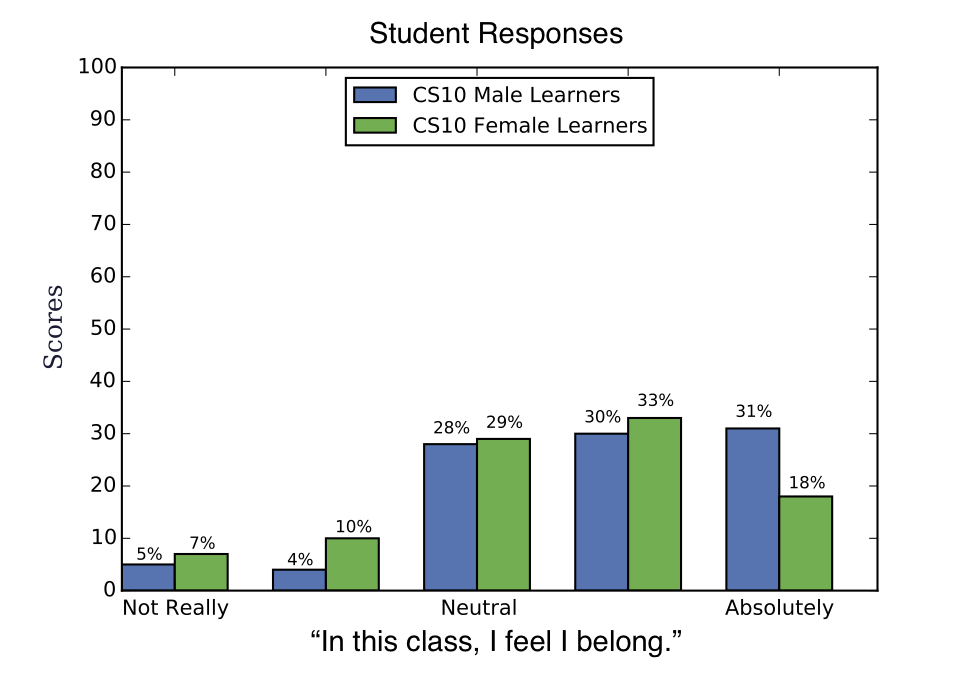
\includegraphics[width=0.5\textwidth]{figures/blg_1_male_female.png}
    \label{blg_1_male_female}}
    \subfloat[]{%
    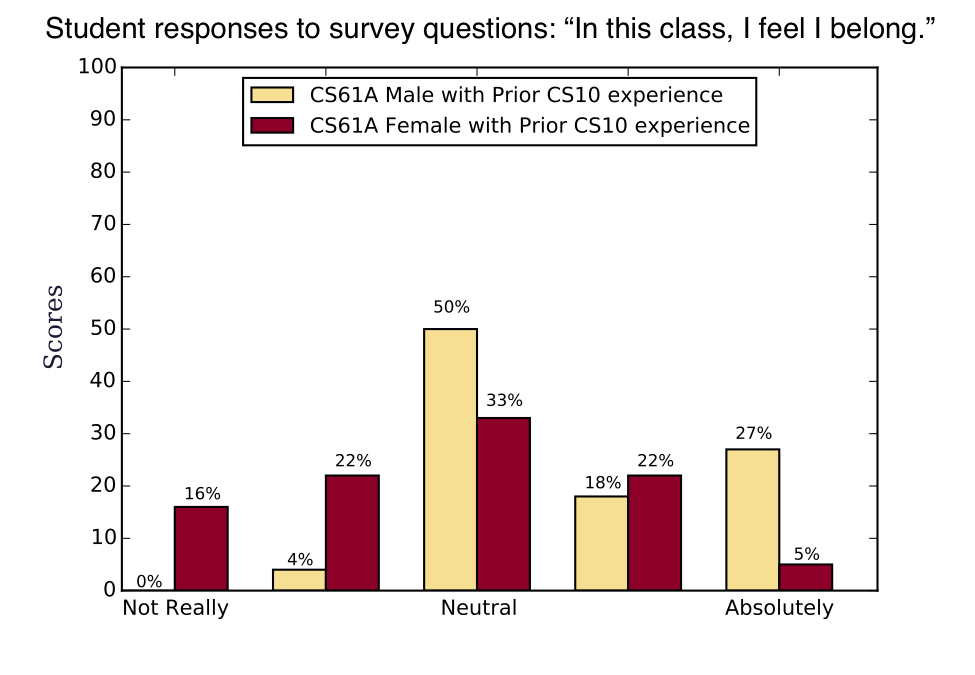
\includegraphics[width=0.5\textwidth]{figures/blg_1_priorcs10.png}
    \label{blg_1_priorcs10}}
  
%
\caption{\textbf{Effects of CS10 on CS61A students' self-reported sense of belonging.}}
\label{fig:blg_1_cs10_cs61a}
\end{figure}


%------------------------------------------------------------------------------------%

\subsubsection *{What impact does CS10 have in attracting female students into the major?}

From the findings in the quantitative analysis, we know that CS10 has a statistically positive effect on female students belief about CS achievement, and in particular, for female students for whom CS10 is their first CS class. If we continue with our working hypothesis that belonging is a strong signifier for a students intention and ability to persist in the major, we can use the instruments constituting that dimension to analyze CS10's ability to attract female students into the major.

To do this, we shift the unit of analysis to the experience of students who had previously attended CS10 and moved on to 61A. When participants were asked the question, ``In this class I feel I belong?,'' The percentage of positive responses went down for female students. The number dropped from 51\% to 27\%. You can see this in figures \ref{blg_1_worstCaseScenario_cs10}, \ref{blg_1_worstCaseScenario}. 

\begin{figure}[!htbp]
    \centering 
    \subfloat[CS10 Learners: blg\_1]{%
    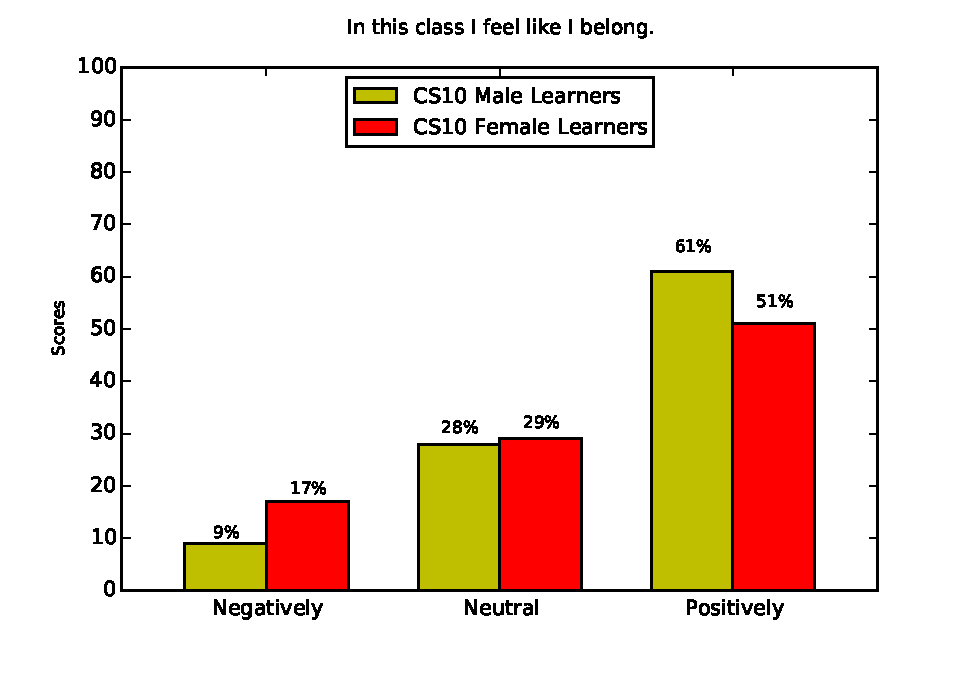
\includegraphics[width=0.5\textwidth]{figures/blg_1_worstCaseScenario_cs10}
    \label{blg_1_worstCaseScenario_cs10}}
    \subfloat[CS61A Learners with \textbf{Prior} CS10: blg\_1]{%
    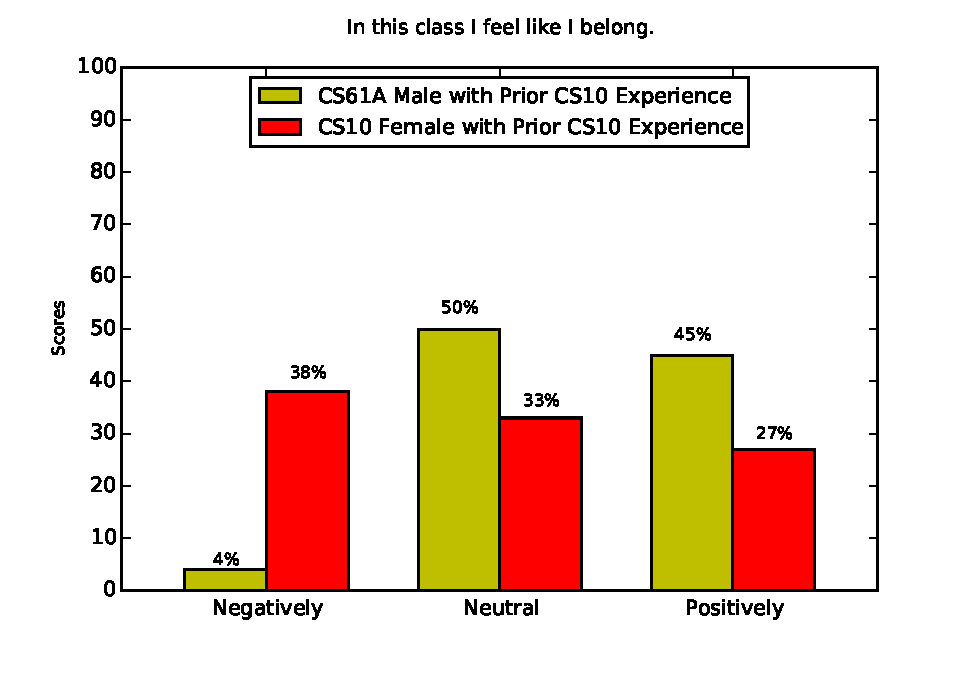
\includegraphics[width=0.5\textwidth]{figures/blg_1_worstCaseScenario}
    \label{blg_1_worstCaseScenario}}
    \qquad
    \subfloat[\textbf{blg\_1}]{%
    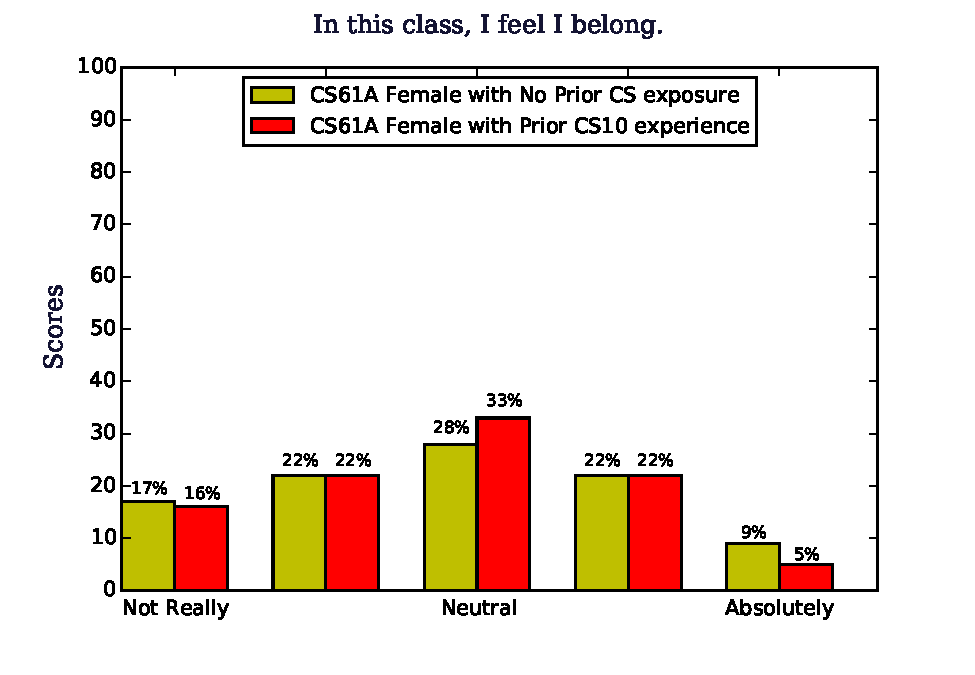
\includegraphics[width=0.5\textwidth]{figures/blg_1_cs10ANDN0_CS}
    \label{fig:blg_1_cs10ANDN0_CS}}
%

%
\caption{\textbf{Effects of CS10 on CS61A students' self-reported sense of belonging.}}
\label{fig:blg_1_cs10_cs61a}
\end{figure}

When comparing the experience of belonging between girls who had never taken any CS, with those of girls who had taken CS10 and then moved on to CS61A, this research found no statistical significance on their experiences. From figure \ref{fig:blg_1_cs10ANDN0_CS}, you can see that the scores are almost the same for both cohort at around 27\% of girls feeling a strong sense of belonging.

In answering the research question, i.e., the ability of belonging in CS10 to predict or say something about an intention to move forward in the introductory CS pipeline, a correlation analysis was conducted on the survey instruments that had to do with computational thinking efficacy, CS efficacy, and belonging. The instruments of particular interest are the following:
\begin{description} 
\item[blg\_1:] In this class, I feel I belong.
\item[blg\_3:] In this class, I feel like my ideas count.
\item[blg\_4:] In this class, I feel like I matter.
\item[atcs\_3:] I can achieve good grades (C or better) in computing courses.
\item[atcs\_8:] I am confident about my abilities with regards to CS.
\item[atct\_5:] I know how to write computer programs.
\item[atct\_8:] I know how to write a computer program to solve a problem.
\end{description}

For the cohort under analysis, i.e., the CS10 female students who went on to CS61A, this study found that for these female students, their self-reported programming ability predicts their sense of belonging, because the correlation heat-map from figure \ref{corrHeatFemale} showed that \textbf{blg\_1} and \textbf{atct\_5} are strongly correlated for girls with (\emph{r}=0.60514), and \textbf{blg\_3} and \textbf{atct\_5} are strongly correlated (\emph{r}=0.63538) \footnote{%
In interpreting correlations, for X and Y values between 0.5 and 0.9, the two variables are strongly related. That is, knowing X allows you to predict Y with considerably greater accuracy than if you didn't know Y. http://sites.stat.psu.edu/~jls/stat100/lectures/lec16.pdf
}. 

\begin{figure}[!htbp]
    \centering
    \subfloat[Female]{%
    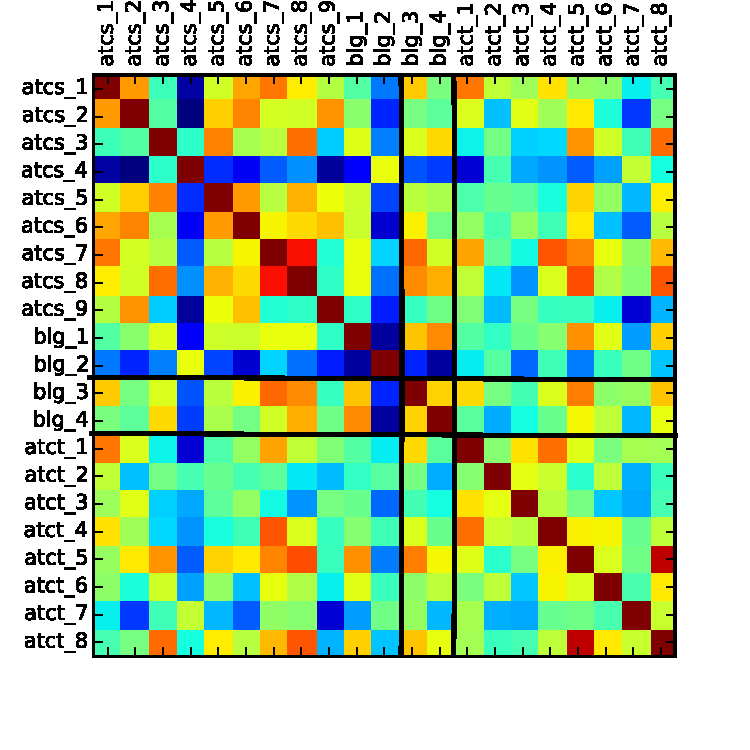
\includegraphics[width=0.5\textwidth]{figures/priorCS10_female_corr}
    \label{corrHeatFemale}}
    \subfloat[Male]{%
    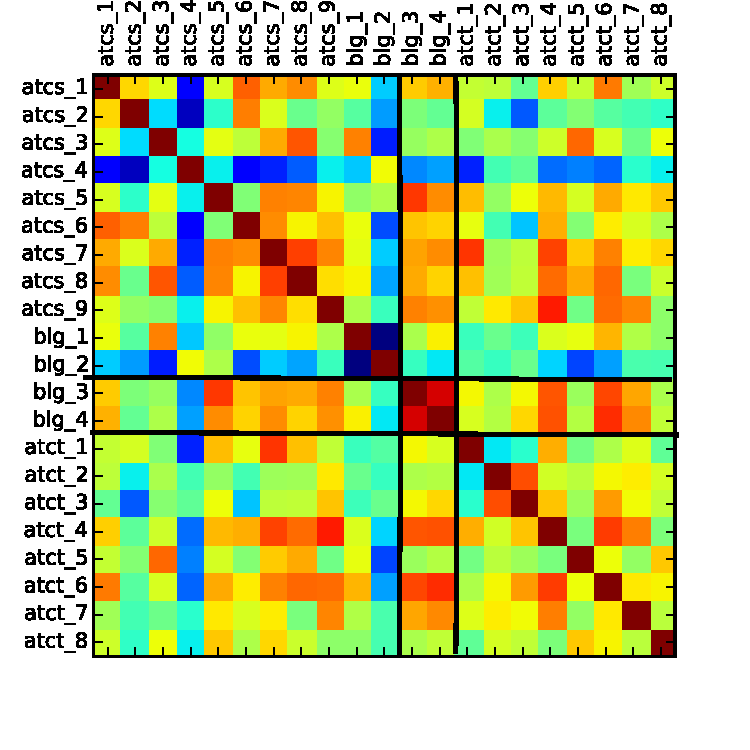
\includegraphics[width=0.5\textwidth]{figures/priorCS10_male_corr}
    \label{corrHeatMale}}
\caption{\textbf{Correlation matrix of CS61A students who had previously taken CS10}}
\label{corrHeatMapFemaleCS10CS61A}
\end{figure}


For male students in the same cohort, this study found something entirely different. From the analysis and from the correlation heat map plotted in figure \ref{corrHeatMale}, we observe that ``\textbf{atct\_4}: I am persistent at solving puzzles or logic problems,'' and ``\textbf{atct\_6}: I am good at building things,'' are strongly correlated with blg\_3 and blg\_4\footnote{ %
blg\_3 \& atct\_4, (\emph{r}=0.70504)\\
blg\_3 \& atcs\_5, (\emph{r}=0.75434)\\
blg\_3 \& atct\_6, (\emph{r}=0.73270)\\
blg\_4 \& atct\_4, (\emph{r}=0.71436)\\
blg\_4 \& atct\_6, (\emph{r}=0.77616)\\
}, with (\emph{r} $\geq$ 0.7) for most of the correlations. 
 
It is important to notice that usually for female CS10 students, based on the raw data spanning three semesters worth of experience, that \textbf{blg\_1} and \textbf{atct\_5} are \emph{not} correlated, (\emph{r}=0.31426), figure \ref{corr_cs10_female}. Since the relationship between these two variables seem to increase as girls move forward in the pipeline, as can be seen from figures \ref{corrHeatMapFemaleCS10CS61A} and \ref{corr_cs61a_female},  we are led to conclude that this relationship is truly a strong predictor of CS belonging. Furthermore, in CS10, the data analysis revealed that female students sense of belonging in that class is highly correlated with their self-reported CS efficacy, as can be seen from the scores in table \ref{corrTab}.

\begin{table}[!htbp]
  \begin{center}
    \begin{tabular}{|p{2cm}|p{2cm}||p{2cm}|}
    \multicolumn{3}{ c }%
    {\textbf{Correlation with Belonging for CS10 Females}}\\[5pt] 
    \hline

    \multicolumn{2}{| c ||}%
    {Instruments} & Score \\[1ex] \hline

    blg\_1 &  atcs\_3 & 0.56885\\
    blg\_1 & atcs\_8 & 0.50070 \\
    blg\_1 & blg\_4 & 0.64547\\
    atct\_5 & atct\_8 & 0.75888 \\

    \hline
    \end{tabular}
    \caption{Correlation Table}
    \label{corrTab}
  \end{center}
\end{table}


When one continues the analysis of the data to focus on the experience of CS10 males and females, as well as CS61A males and females, more insight is revealed on the self-reported attitudes of the students in the introductory to CS pipeline.

From figure \ref{corr_cs10_male}, we can see that the males in CS10 are the only subset in the study that do not have their sense of belonging correlated with their CS efficacy or their computational thinking (CT) efficacy, where as all the other subsets do as can be seen from figures \ref{corr_cs10_female}, \ref{corr_cs61a_female} and \ref{corr_cs61a_male}. However, once the gentlemen move on from CS10 to CS61A, from the data analysis, we find that their sense of belonging starts getting correlated with CS and CT efficacy, as can be seen from figure \ref{corrHeatMale}.

\begin{figure}[!htbp]
    \centering
    \subfloat[CS10]{%
    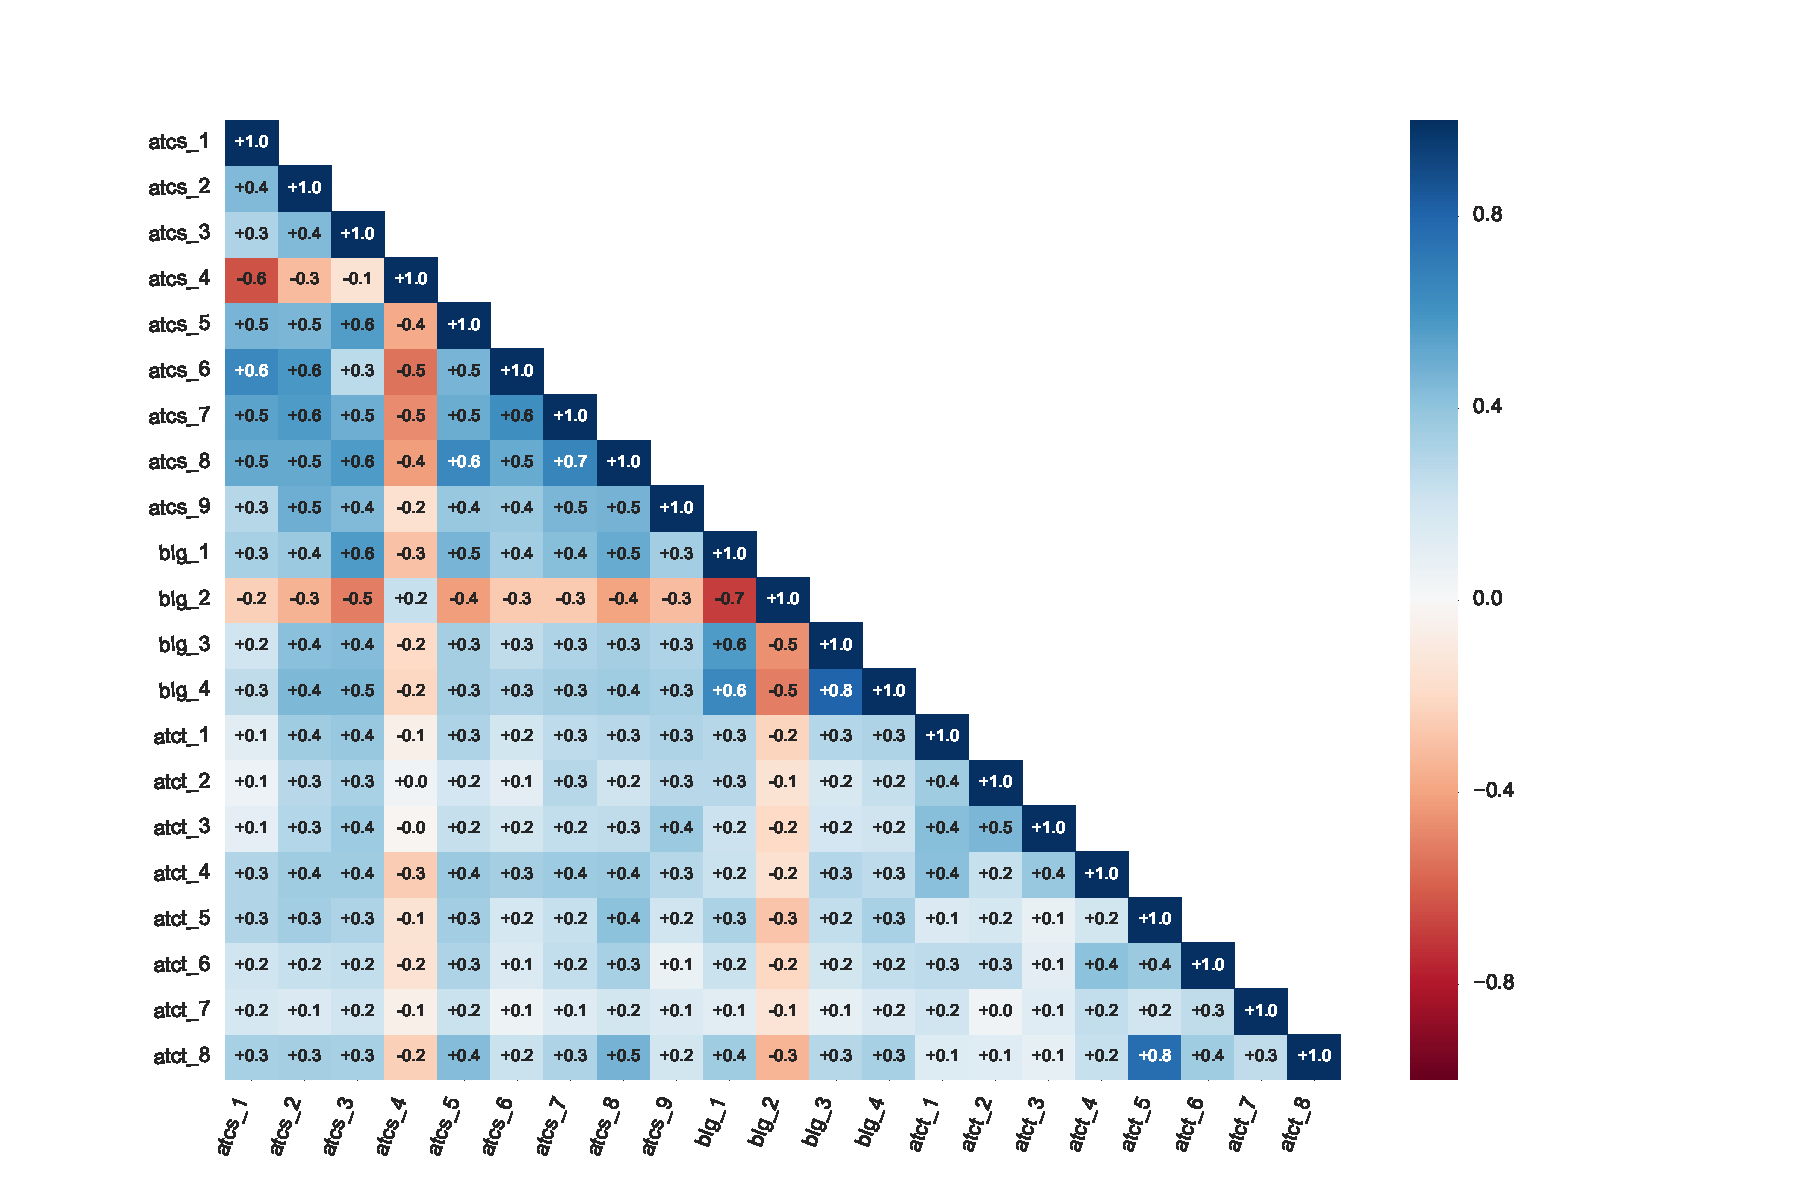
\includegraphics[width=0.5\textwidth]{figures/cs10_female_corr}
    \label{corr_cs10_female}}
    \subfloat[CS61A]{%
    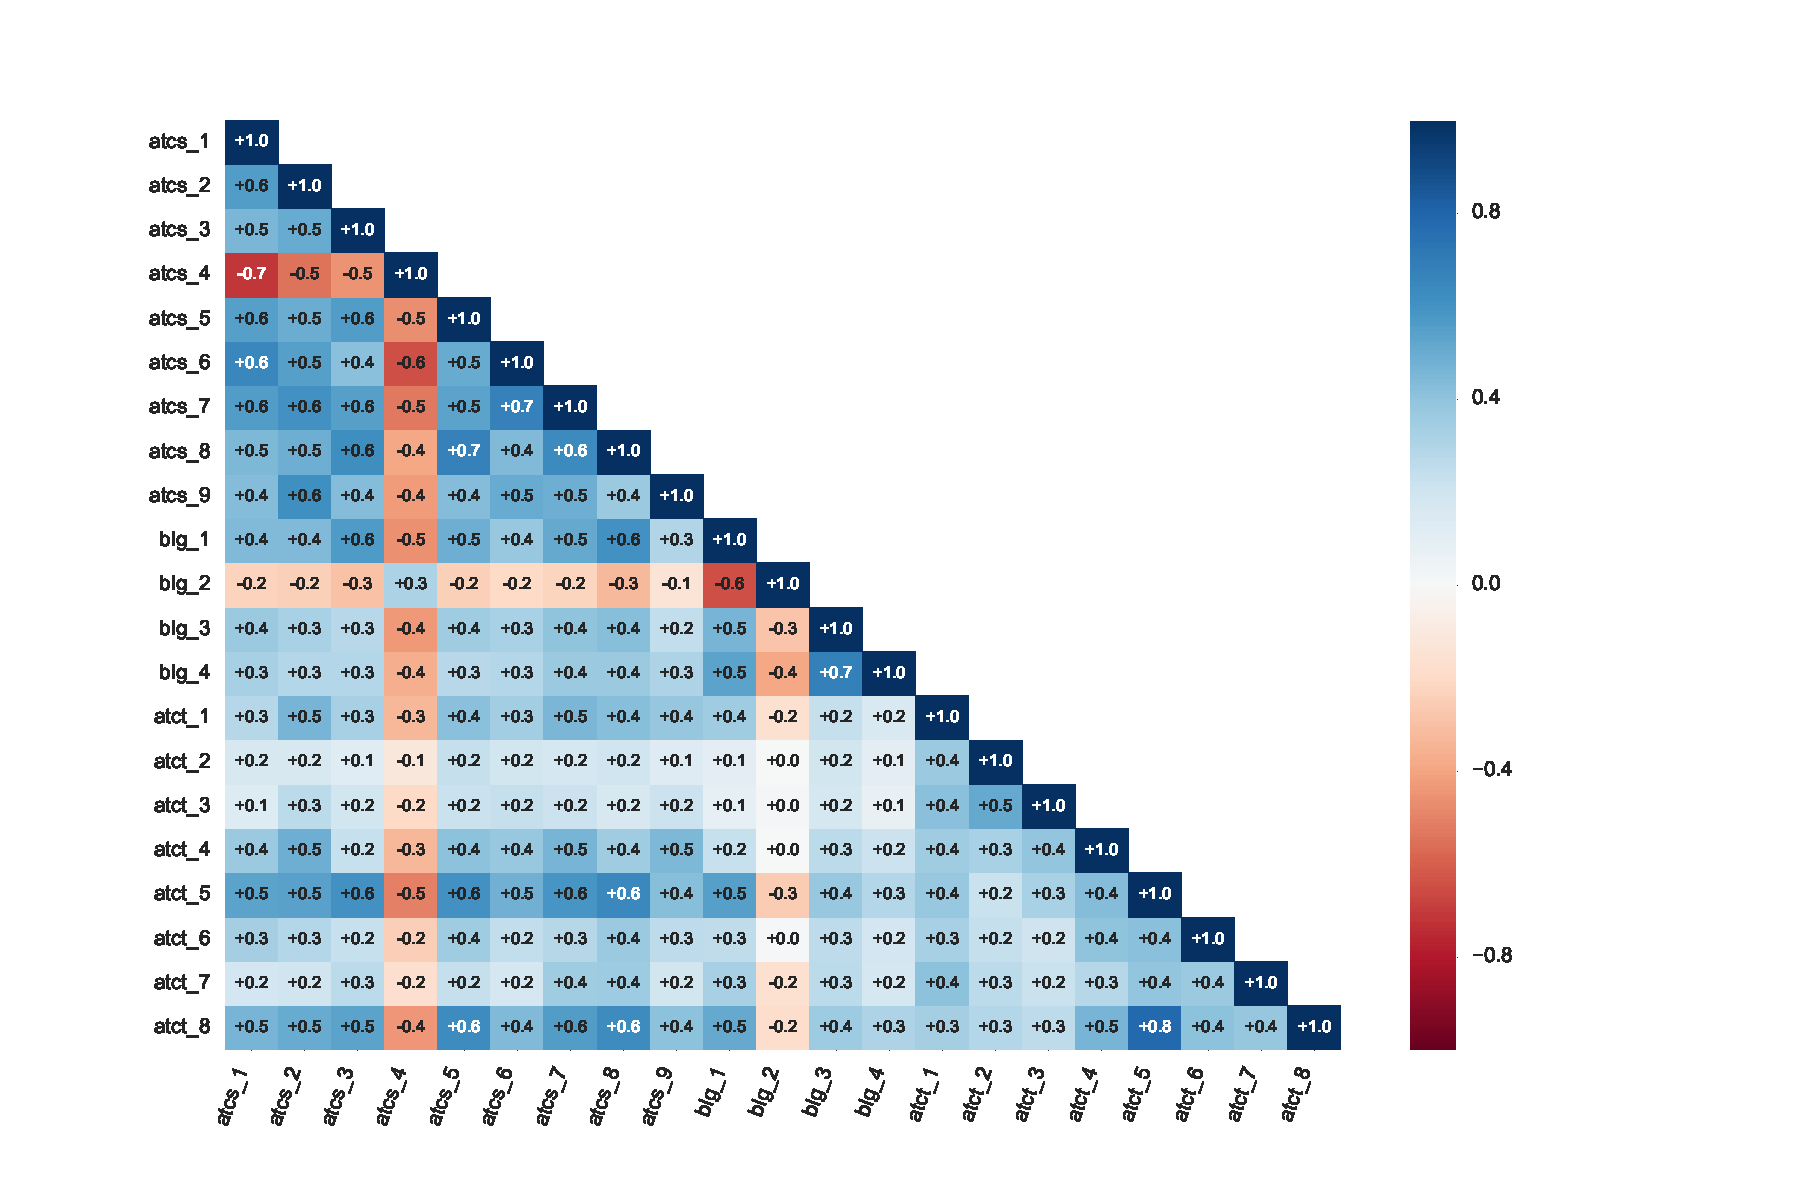
\includegraphics[width=0.5\textwidth]{figures/cs61a_female_corr}
    \label{corr_cs61a_female}}
%
\caption {\textbf{Correlation matrix for female students in intro CS at UC Berkeley}}
\label{fig:corrFemale}
\end{figure}

\begin{figure}[!htbp]
    \centering
    \subfloat[CS10]{%
    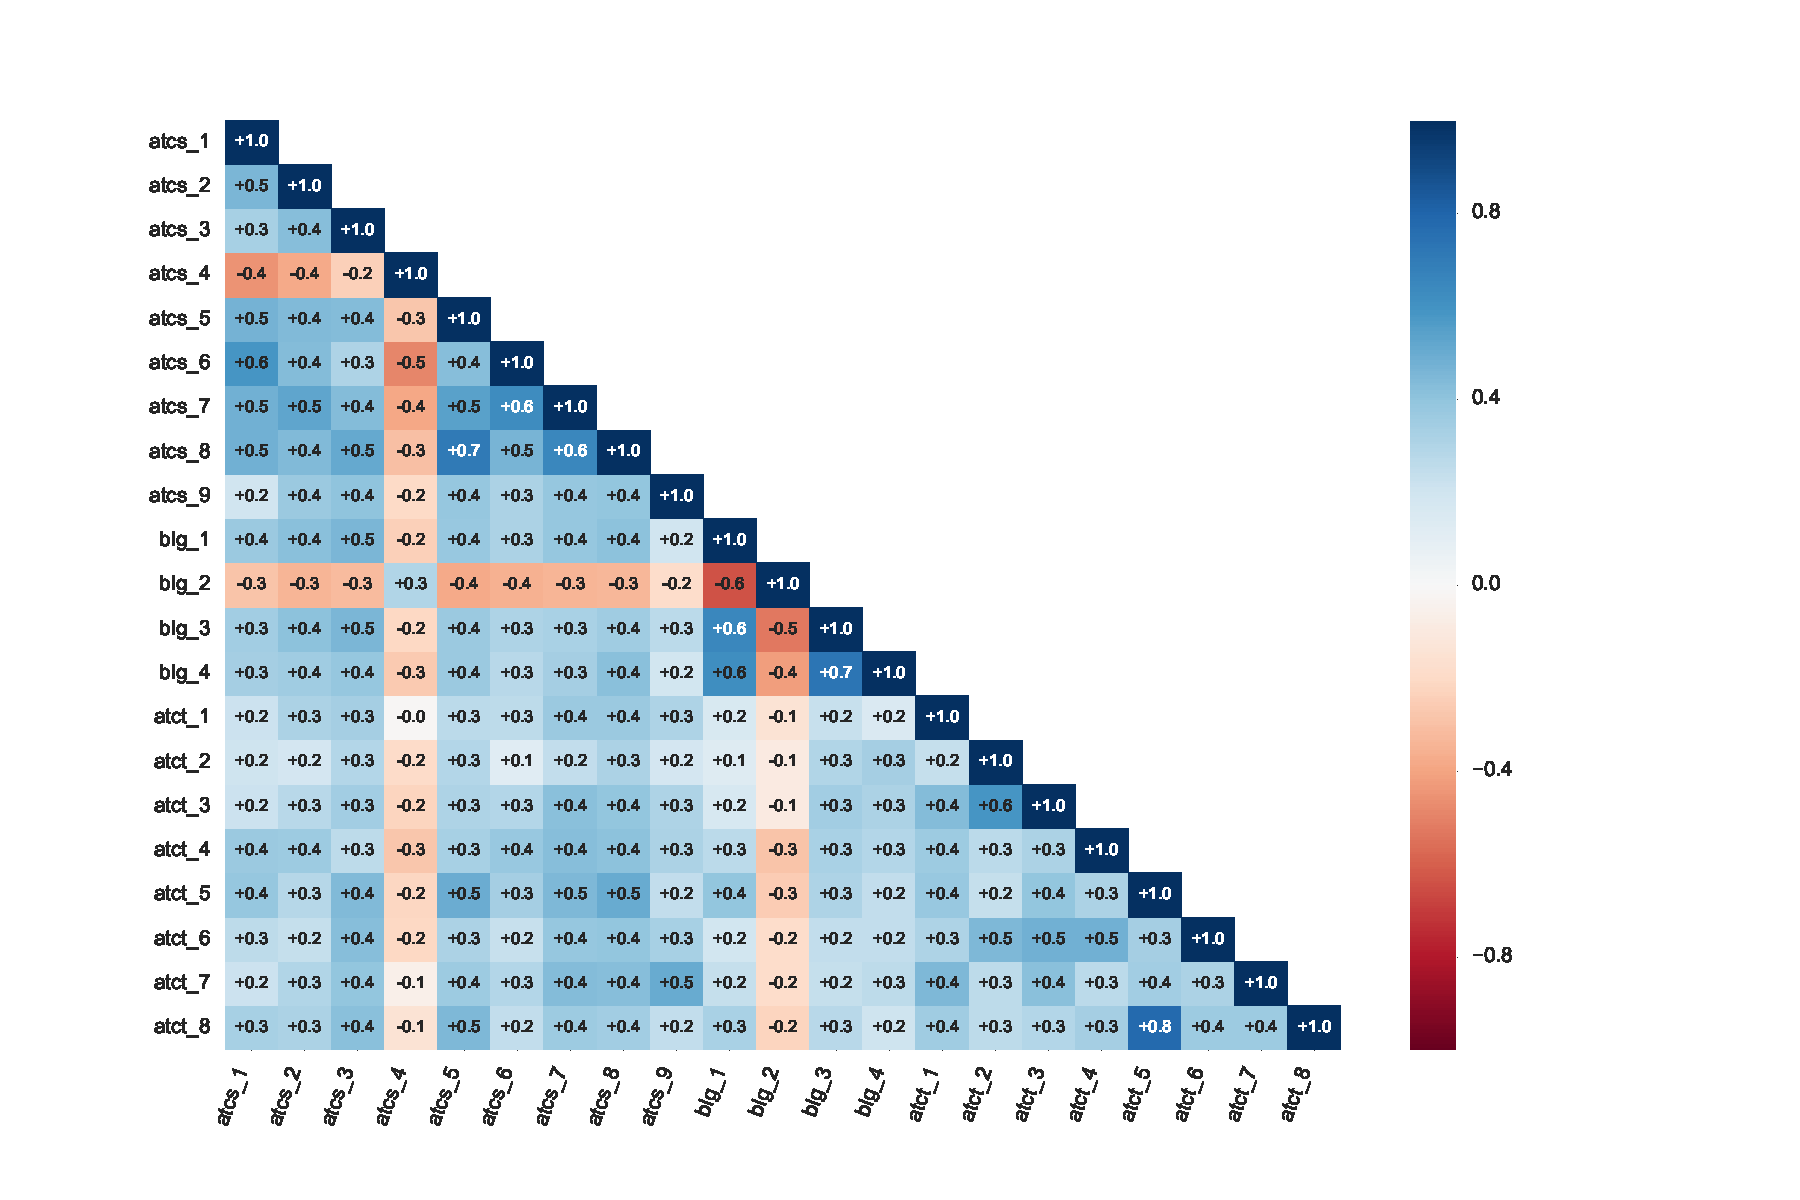
\includegraphics[width=0.5\textwidth]{figures/cs10_male_corr}
    \label{corr_cs10_male}}
    \subfloat[CS61A]{%
    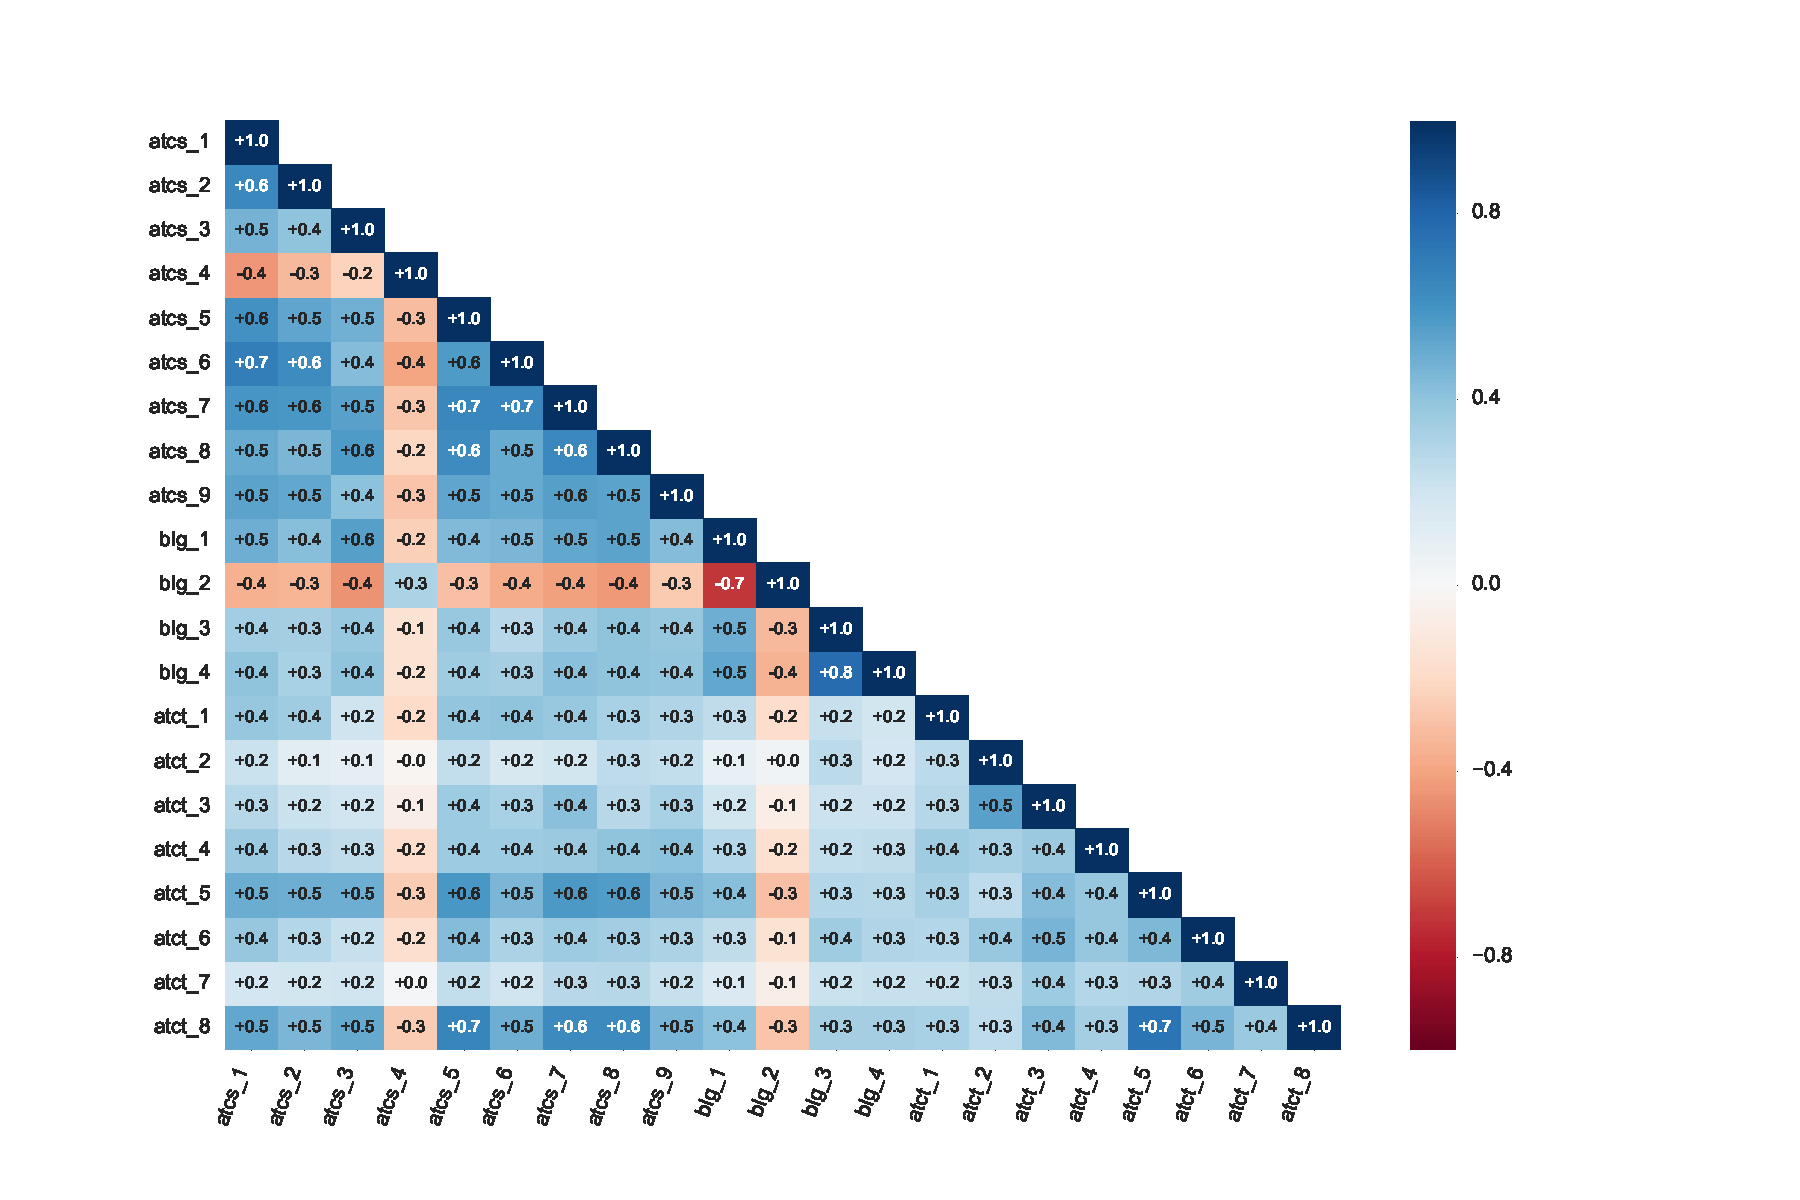
\includegraphics[width=0.5\textwidth]{figures/cs61a_male_corr}
    \label{corr_cs61a_male}}   
%
\caption {\textbf{Correlation matrix for male students in intro CS at UC Berkeley}}
\label{fig:corrMale}
\end{figure}

 


%----------------------------------------------------------------------------------------
\section*{Conclusion}

This paper has laid out some of the challenge of equalizing participation in CS. A mixed-methods formative research was conducted that sought to to answer the question, ``What are the socio-curricular factors that lead historically underrepresented students to choose CS?'' Findings from the formative mixed-method research which demonstrated the efficacy of socio-cultural, responsive, curriculum in broadening participation in CS was put forth. 


From the findings in the quantitative analysis, we know that CS10 has a statistically positive effect on female students belief about CS achievement, and in particular, for female students for whom CS10 is their first CS class. Furthermore, for the CS10 female students who went on to CS61A, this study found that for these students, their self-reported programming ability predicts their sense of belonging. 

While CS10 is successfully serving as a gateway into the major for underrepresented students, from the analysis, as great a class as CS10 is, there are still some significant environmental challenges that the overwhelmingly male environment of CS61A poses to female students sense of belonging when they advance on to 61A.

The hope is that as like-minded-people continue to work in this area of equalizing participation in CS, maybe she can finally be the radical, innovative field she has always said she was---by bringing about a different way of life for the 21st century. 


% Back pages ==================================================================

% Bibliography ================================================================

\chapter{References}

\begingroup
    \def\chapter*#1{}
    \bibliographystyle{abbrvnat}
    \renewcommand{\bibname}{}
    \label{app:bibliography}
    \bibliography{bibliography}
\endgroup


\end{document}  